% Copyright 2004 by Till Tantau <tantau@users.sourceforge.net>.
%
% In principle, this file can be redistributed and/or modified under
% the terms of the GNU Public License, version 2.
%
% However, this file is supposed to be a template to be modified
% for your own needs. For this reason, if you use this file as a
% template and not specifically distribute it as part of a another
% package/program, I grant the extra permission to freely copy and
% modify this file as you see fit and even to delete this copyright
% notice. 
\documentclass{beamer}

\usepackage{graphicx}
\graphicspath{{./images/}}
\usepackage{pgf-pie}
\usepackage{amsmath}
\usepackage{wrapfig}

\usepackage{hyperref}
%\usepackage{xcolor}

\usepackage{subcaption}

\usepackage{smartdiagram}

\usepackage[backend=bibtex,style=authoryear,natbib=true]{biblatex} % Use the bibtex backend with the authoryear citation style (which resembles APA)

\addbibresource{retinopathy.bib} % The filename of the bibliography


% There are many different themes available for Beamer. A comprehensive
% list with examples is given here:
% http://deic.uab.es/~iblanes/beamer_gallery/index_by_theme.html
% You can uncomment the themes below if you would like to use a different
% one:
%\usetheme{AnnArbor}
%\usetheme{Antibes}
%\usetheme{Bergen}
%\usetheme{Berkeley}
%\usetheme{Berlin}
%\usetheme{Boadilla}
%\usetheme{boxes}
%\usetheme{CambridgeUS}
%\usetheme{Copenhagen}
%\usetheme{Darmstadt}
%\usetheme{default}
%\usetheme{Frankfurt}
%\usetheme{Goettingen}
%\usetheme{Hannover}
%\usetheme{Ilmenau}
%\usetheme{JuanLesPins}
%\usetheme{Luebeck}
\usetheme{Madrid}
%\usetheme{Malmoe}
%\usetheme{Marburg}
%\usetheme{Montpellier}
%\usetheme{PaloAlto}
%\usetheme{Pittsburgh}
%\usetheme{Rochester}
%\usetheme{Singapore}
%\usetheme{Szeged}
%\usetheme{Warsaw}

% Change base colour beamer@blendedblue (originally RGB: 0.2,0.2,0.7)
%\colorlet{beamer@blendedblue}{red!40!black}

\usecolortheme{dolphin}
% default albatross beaver beetle crane dolphin 
% dove fly lily orchid rose seagull seahorse whale wolverine

%  The outertheme defines the head and the footline of each slide. 

%\useoutertheme{infolines}
% infolines miniframes shadow sidebar smoothbars 
% smoothtree split tree

%\useinnertheme{rectangles}
% rectangles circles inmargin rounded

\title[Ph.D. Thesis Presentation]{Diabetic Retinopathy Classification and Interpretation using Deep Learning Techniques}

% A subtitle is optional and this may be deleted
%\subtitle{}

\author{Jordi de la Torre} %\and S.~Another\inst{2}}
% - Give the names in the same order as the appear in the paper.
% - Use the \inst{?} command only if the authors have different
%   affiliation.

\institute[URV] % (optional, but mostly needed)
{
  %\inst{1}%
  Doctorate Program of Computer Science and Mathematics of Security\\
  Supervisors: Dra. A\"ida Valls and Dr. Dom\`enec Puig\\
  Universitat Rovira i Virgili}
  %\and
  %\inst{2}%
  %Department of Theoretical Philosophy\\
  %University of Elsewhere}
% - Use the \inst command only if there are several affiliations.
% - Keep it simple, no one is interested in your street address.

\date{March 12, 2019}
% - Either use conference name or its abbreviation.
% - Not really informative to the audience, more for people (including
%   yourself) who are reading the slides online

\subject{Computer Science}
% This is only inserted into the PDF information catalog. Can be left
% out. 

% If you have a file called "university-logo-filename.xxx", where xxx
% is a graphic format that can be processed by latex or pdflatex,
% resp., then you can add a logo as follows:

\pgfdeclareimage[height=0.3cm]{itaka}{itaka.png}
\pgfdeclareimage[height=0.3cm]{rivi}{rivi.png}
\pgfdeclareimage[height=0.5cm]{urv}{urv.jpg}
\logo{\pgfuseimage{itaka}\pgfuseimage{rivi}\pgfuseimage{urv}}

\AtBeginPart{\frame{\partpage}}

\AtBeginSection[]
{
	\begin{frame}<beamer>{Outline}
	%\tableofcontents[currentsection,hideothersubsections]
	\tableofcontents[currentsection,currentsubsection]
\end{frame}
}


% Delete this, if you do not want the table of contents to pop up at
% the beginning of each subsection:
%\AtBeginSubsection[]
%{
%  \begin{frame}<beamer>{Outline}
%    \tableofcontents[currentsection,currentsubsection]
%  \end{frame}
%}


% Section and subsections will appear in the presentation overview
% and table of contents.

% Let's get started
\begin{document}

\begin{frame}
  \titlepage
\end{frame}

\section*{Outlines}

\begin{frame}{Outline}
\begin{columns}
	\begin{column}{0.5\textwidth}
		\underline{Part 1 - Introduction}
		\tableofcontents[part={1},hideothersubsections]
		\hfill \break
		\underline{Part 2 - Classification}
		\tableofcontents[part={2},hideothersubsections]
	\end{column}
	\begin{column}{0.5\textwidth}
		\underline{Part 3 - Interpretation}
		\tableofcontents[part={3},hideothersubsections]
		\hfill \break
		\underline{Part 4 - Conclusions}
		\tableofcontents[part={4},hideothersubsections]
	\end{column}
\end{columns}
\end{frame}

%\subsection{Part I: Introduction and Background}
%\frame{
%	\frametitle{Outline - Part of Introduction and Background}
%	\tableofcontents[part={1}]}
%\subsection{Part II: Classification}
%\frame{
%	\frametitle{Outline - Part of Classification}
%	\tableofcontents[part={2}]}
%\subsection{Part III: Interpretation}
%\frame{
%	\frametitle{Outline - Part of Interpretation}
%	\tableofcontents[part={3}]}
%\subsection{Part IV: Application and Conclusions}
%\frame{
%	\frametitle{Outline - Part of Conclusions}
%	\tableofcontents[part={4}]}

\part{Introduction and Background}

\section{Introduction and Background}

\subsection{Objectives}

\begin{frame}{Thesis Objective}
\centering
\Large Design a self-explainable method for automatic diabetic retinopathy disease grading, based on the analysis of retina fundus images with an accuracy close to the human experts in the field.

\end{frame}


%\subsection{Motivation}

%\begin{frame}{Motivation}{}
%\begin{columns}
%	\begin{column}{0.6\textwidth}
%		\begin{itemize}
%			\item {Diabetic Retinopathy (DR) is a leading disabling chronic disease.}
%%			\item {Main cause of blindness and visual impairment in developed countries for diabetic patients.}
%			\item{Diagnostic automation can help the physicians to improve the quality of their diagnostics and reduce the cost associated with it.}
%		\end{itemize}	
%	\end{column}
%	\begin{column}{0.4\textwidth}  %%<--- here
%		\begin{figure}[p]
%			\centering
%			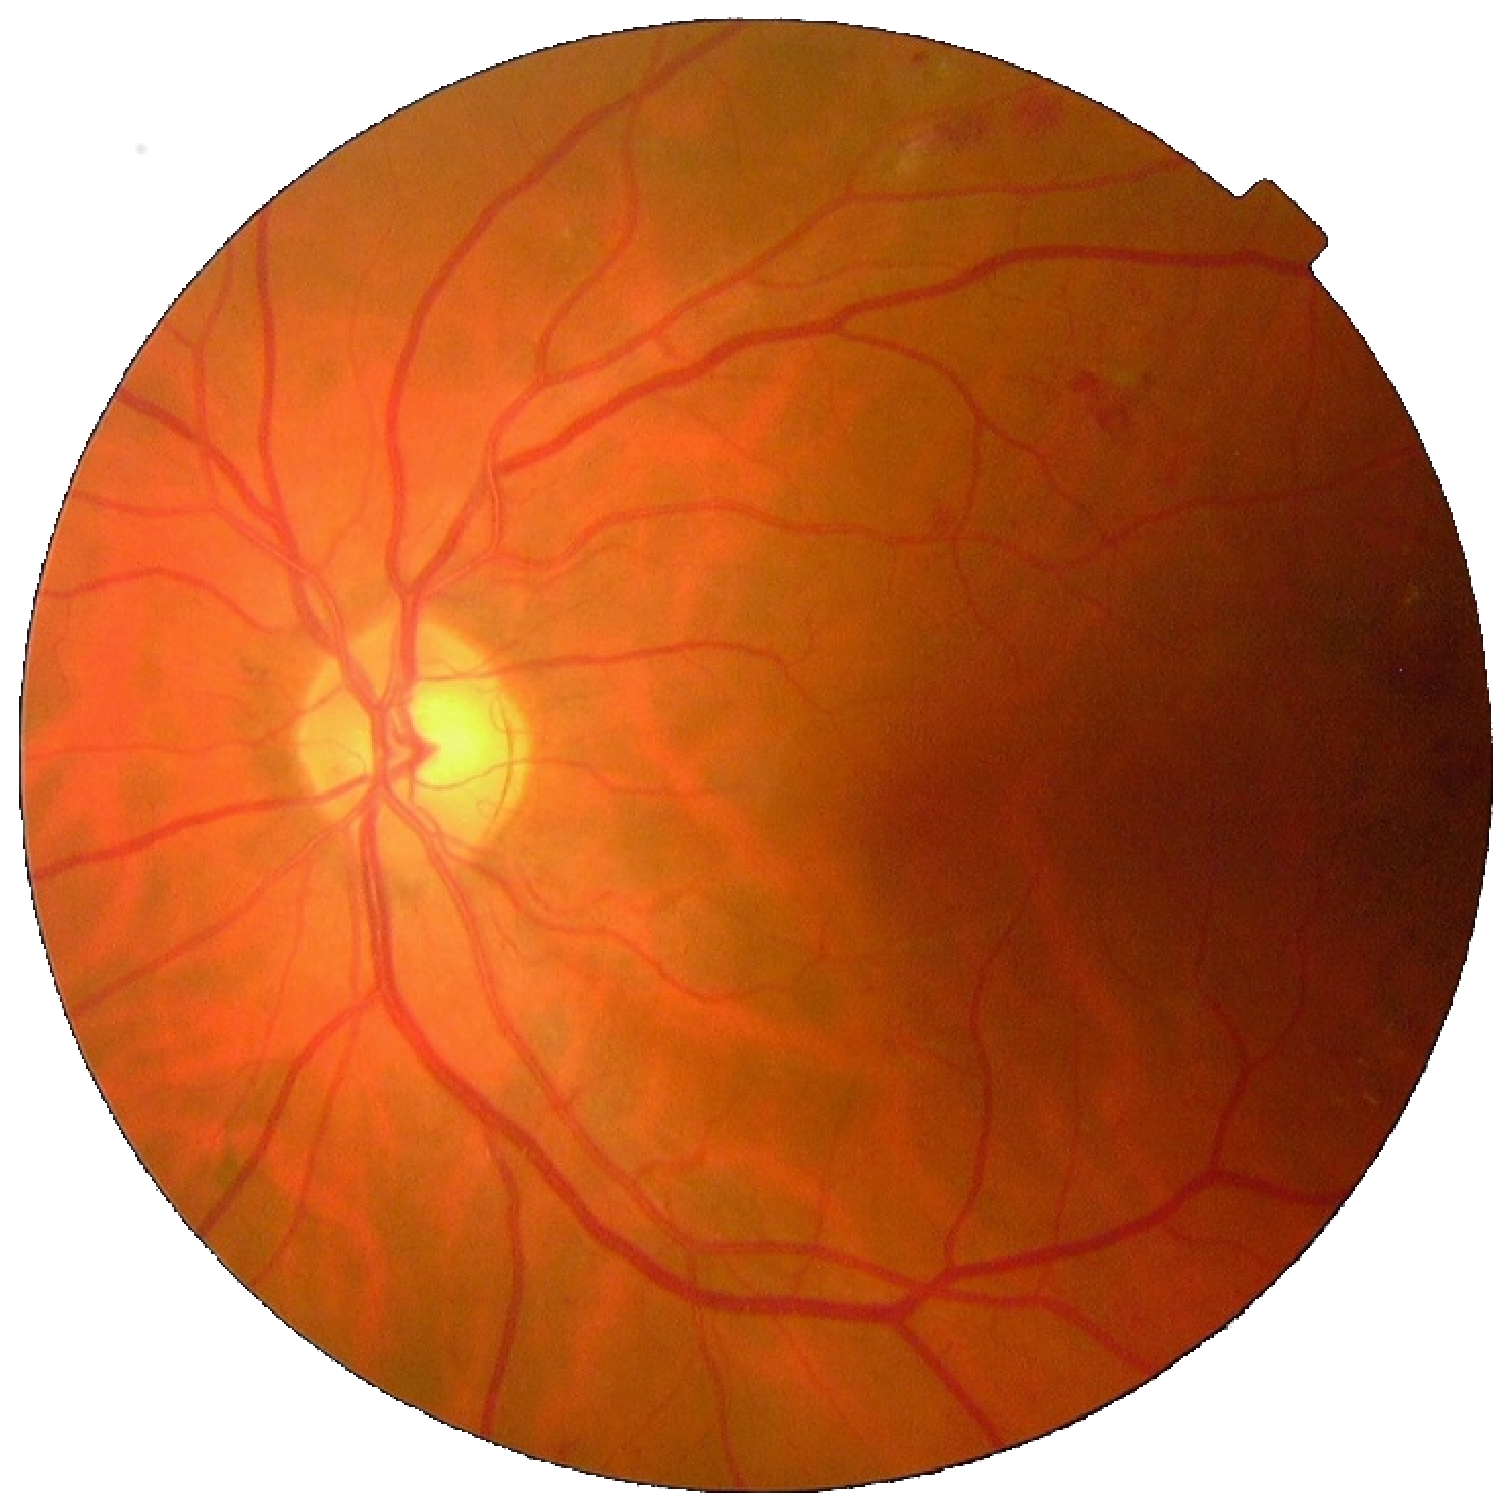
\includegraphics[width=\textwidth]{retine.eps}
			%\caption{Image taken with a non-mydriatic fundus camera.}
%		\end{figure}
%	\end{column}
%\end{columns}

%\end{frame}



%\section{Background}

\subsection{Diabetic Retinopathy}

\begin{frame}{Diabetic Retinopathy}{Eye Structure}
\begin{columns}
	\begin{column}{0.6\textwidth}
		\begin{itemize}
			\item {Light passes through the cornea, iris and lens reaching the internal structures of the eye.}
			\item {It impacts the back of the eye, where retina is located.}
			\item{Light activates a set of sensory elements in retina.}
			\item{The signal of these sensory elements is transported through the optic nerve to the brain.}
		\end{itemize}	
	\end{column}
	\begin{column}{0.4\textwidth}  %%<--- here
		\begin{figure}[p]
			\centering
			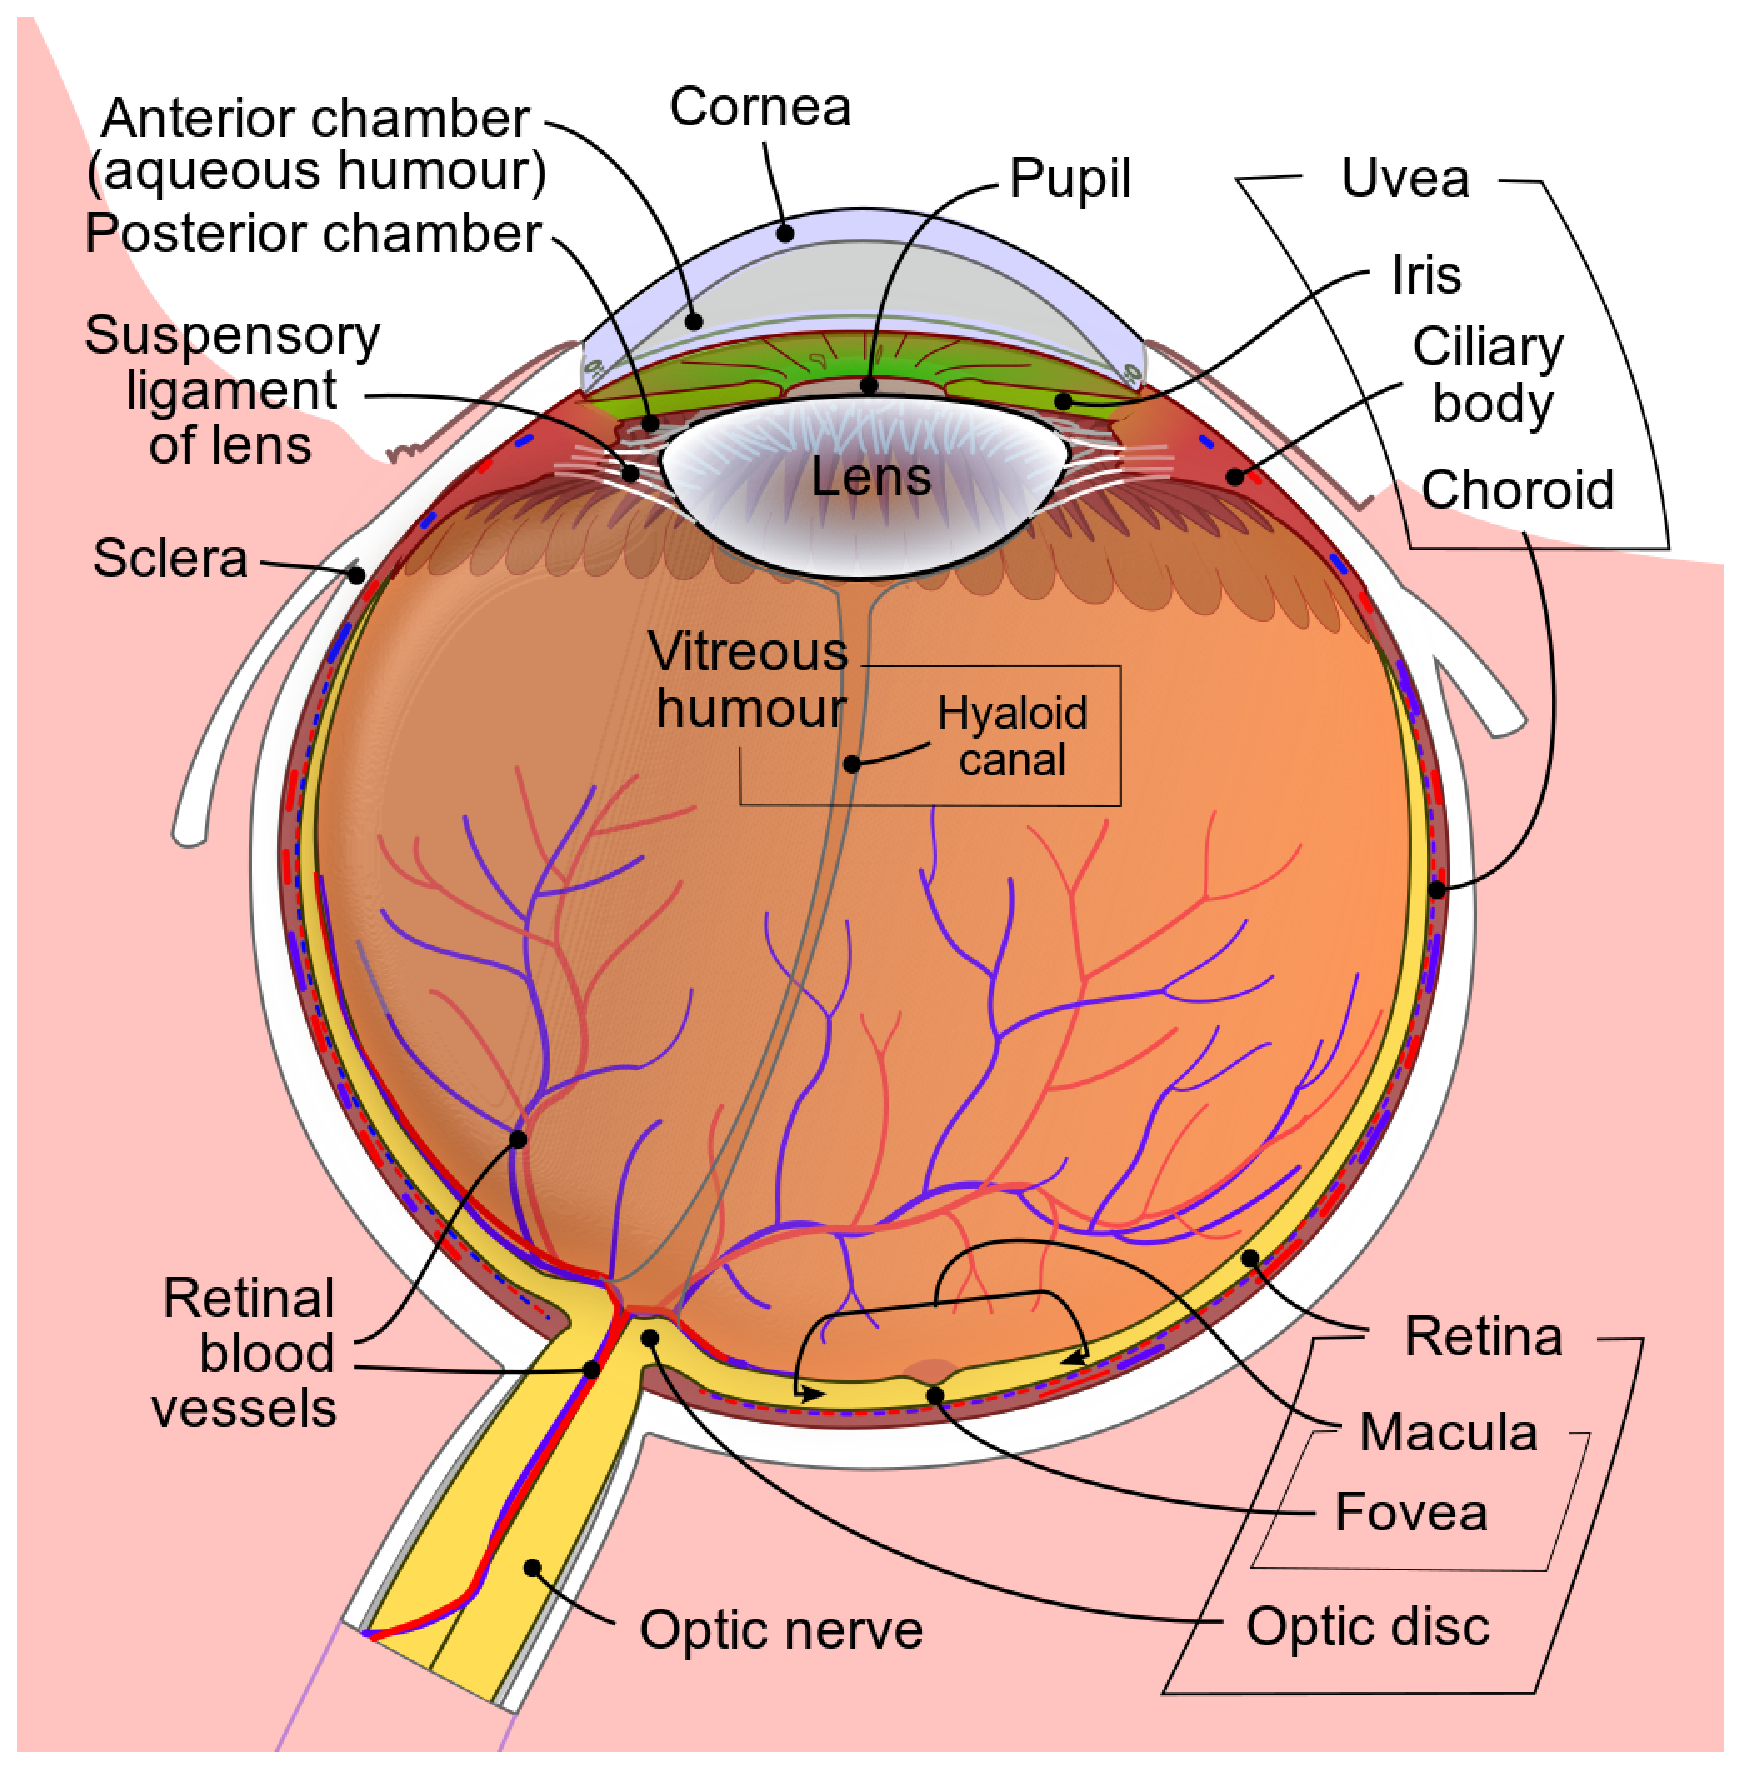
\includegraphics[width=\textwidth]{eye_en.eps}
			%\caption{Image taken with a non-mydriatic fundus camera.}
		\end{figure}
	\end{column}
\end{columns}
\end{frame}

\begin{frame}{Diabetic Retinopathy}{What diabetic retinopathy is?}
\begin{columns}
	\begin{column}{0.5\textwidth}
		\begin{itemize}
			\item {Disease derived from diabetic condition.}
			\item{Affects to the sensory elements of the retina.}
			\item{Produced by the deterioration of retina irrigation capilars.}
			\item{If not treated, it can cause vision quality loss and eventually blindness.}
			\item{Typical lesions: microaneurysms, "cotton wool" spots, abnormal neovascularization, hemorrhages. }
		\end{itemize}	
	\end{column}
	\begin{column}{0.5\textwidth}  %%<--- here
		\begin{figure}[p]
			\centering
			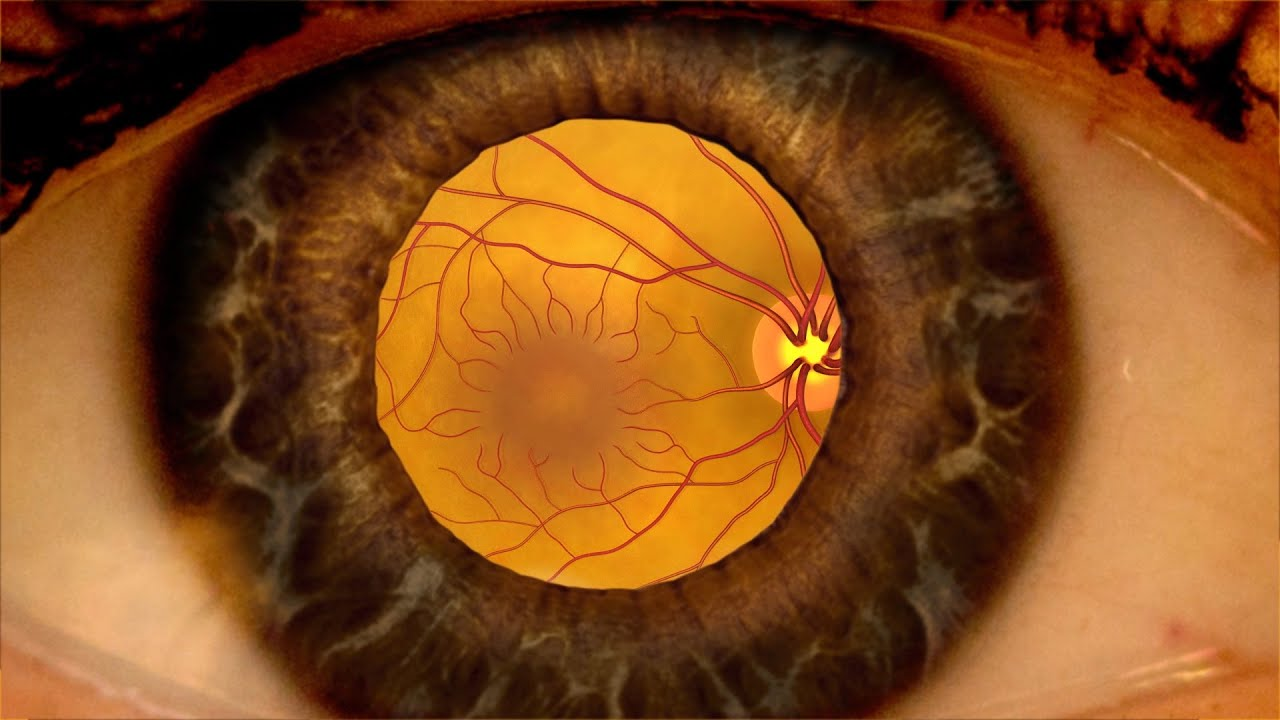
\includegraphics[width=0.7\textwidth]{eye_dilated_pupil_retina.jpg}
			\\
			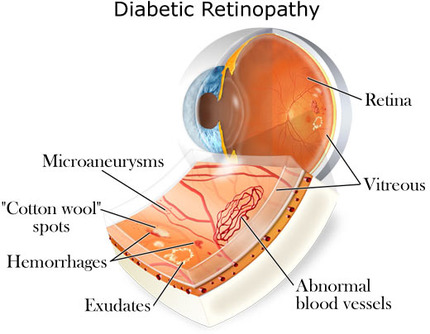
\includegraphics[width=0.9\textwidth]{DiabeticRetinopathy_431x334.jpg}
		\end{figure}
	\end{column}
\end{columns}
\end{frame}

\begin{frame}{Diabetic Retinopathy}{Evaluation Technique: Fundus photography}
It allows the visualization of main structures present in the back of eye interior.
\begin{figure}[p]
\centering
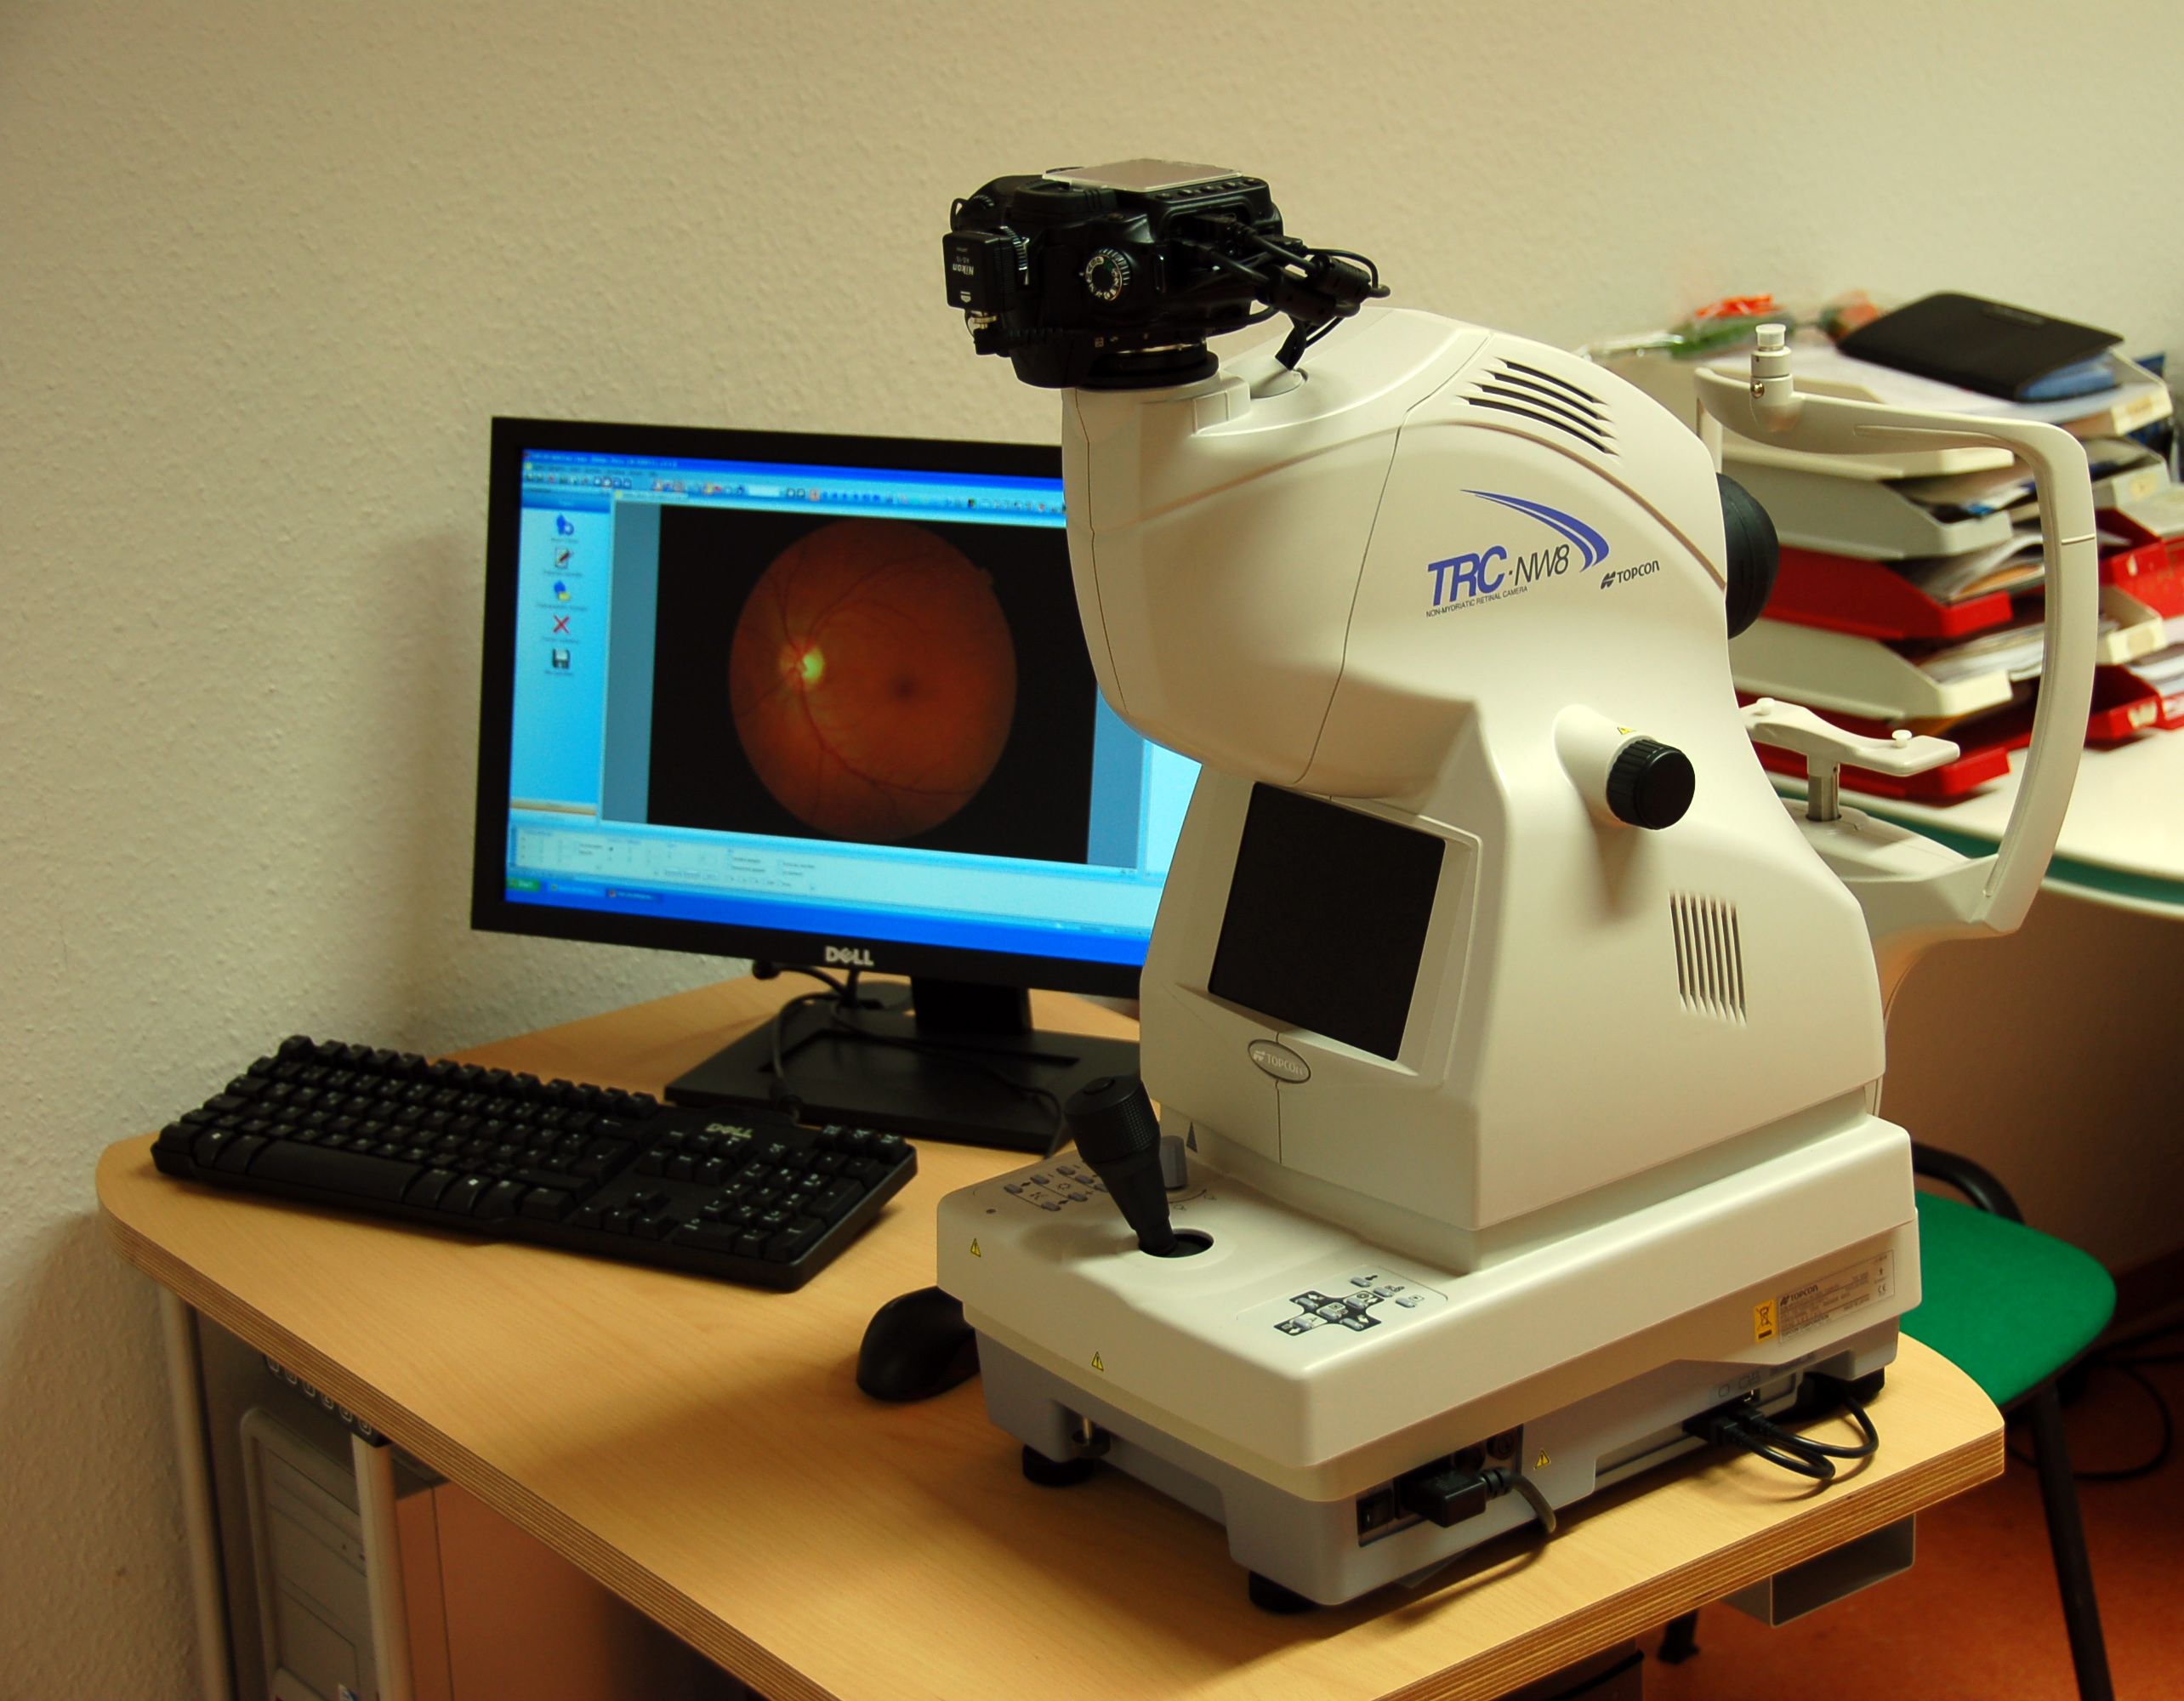
\includegraphics[width=0.65\textwidth]{fundus_camera.jpg}
%\caption{Image taken with a non-mydriatic fundus camera.}
\end{figure}
\end{frame}

%\begin{frame}{Retinal Typical Images}{}
%\begin{figure}[p]
%\centering
%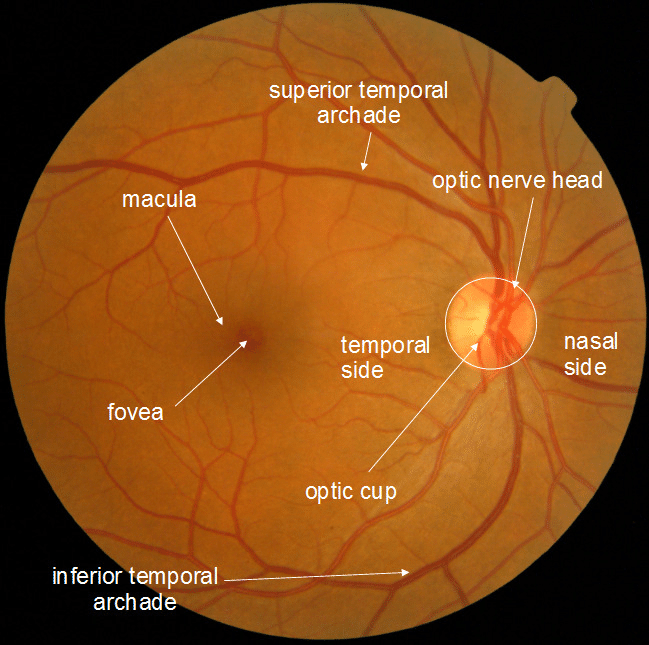
\includegraphics[width=0.65\textwidth]{2-NM-1-field-image-with-labeled-retinal-landmarks.png}
%\caption{Image taken with a non-mydriatic fundus camera.}
%\end{figure}
%\end{frame}

\begin{frame}{Diabetic Retinopathy}{Typical DR lesions}
\begin{figure}[p]
	\centering
	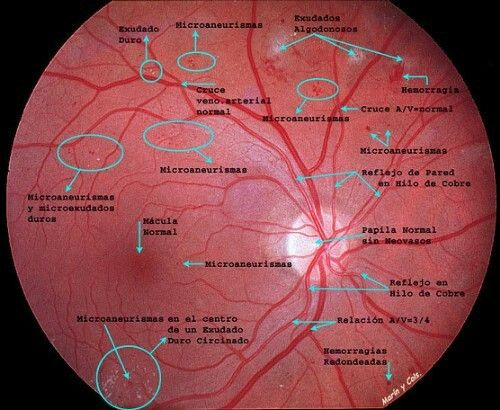
\includegraphics[width=0.80\textwidth]{diabetic-retinopathy-typical-lesions.jpg}
	%\caption{Image taken with a non-mydriatic fundus camera.}
\end{figure}
\end{frame}


\begin{frame}{Diabetic Retinopathy Grade Classification}{Grading table}
\begin{figure}[p]
	\centering
	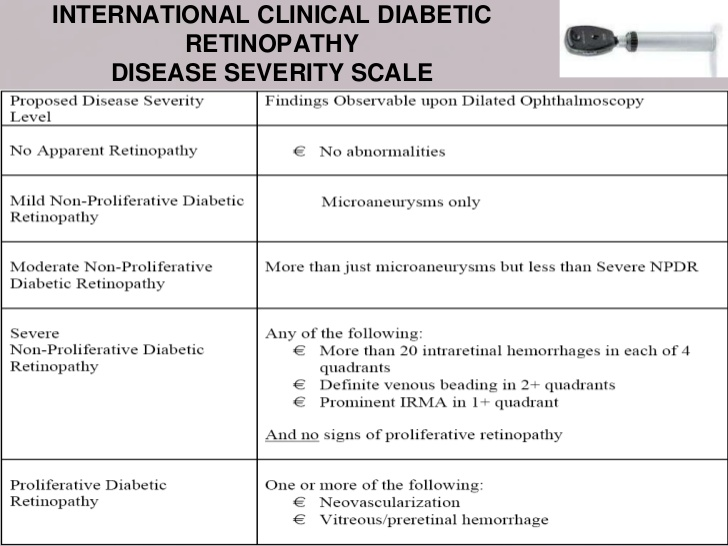
\includegraphics[width=0.85\textwidth]{diabetic-retinopathy-grading-table.jpg}
	%\caption{Image taken with a non-mydriatic fundus camera.}
\end{figure}
\end{frame}

%\begin{frame}{Diabetic Retinopathy}{Grade Classification}
%\begin{figure}[p]
%	\centering
%	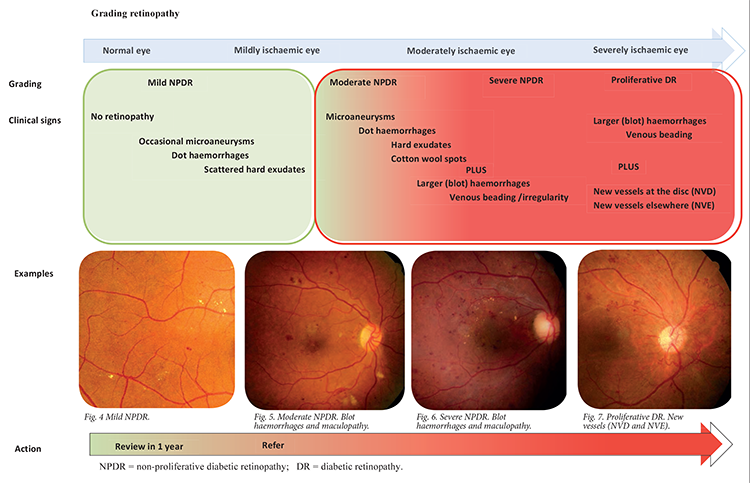
\includegraphics[width=0.80\textwidth]{image_DR_disease_grades.png}
	%\caption{Image taken with a non-mydriatic fundus camera.}
%\end{figure}
%\tiny \fullcite{CME2643}
%\end{frame}

%\begin{frame}{Diabetic Retinopathy Grade Classification}{Summary}
%\begin{itemize}
%	\item {Classification of retina images into 5 different categories of increasing disease grade.}
%	\item {It is a standardized classification defined by ophthalmologists: \scriptsize \fullcite{diaclass}}
%\end{itemize}
%\begin{figure}[p]
%	\includegraphics[width=0.9\textwidth]{classes.eps}
%	\caption{Five samples of increasing grade. From left to right: 0, no apparent DR; 1, mild non-proliferative (NPDR); 2, moderate NPDR; 3, severe NPDR and 4, proliferative DR}
%\end{figure}	
%\end{frame}


\subsection{Evaluation Measures}

\begin{frame}{Evaluation Measures}{Binary Classification}
Evaluation Methods used for binary classification when a "true gold standard" is available:
\begin{figure}[p]
	\centering
	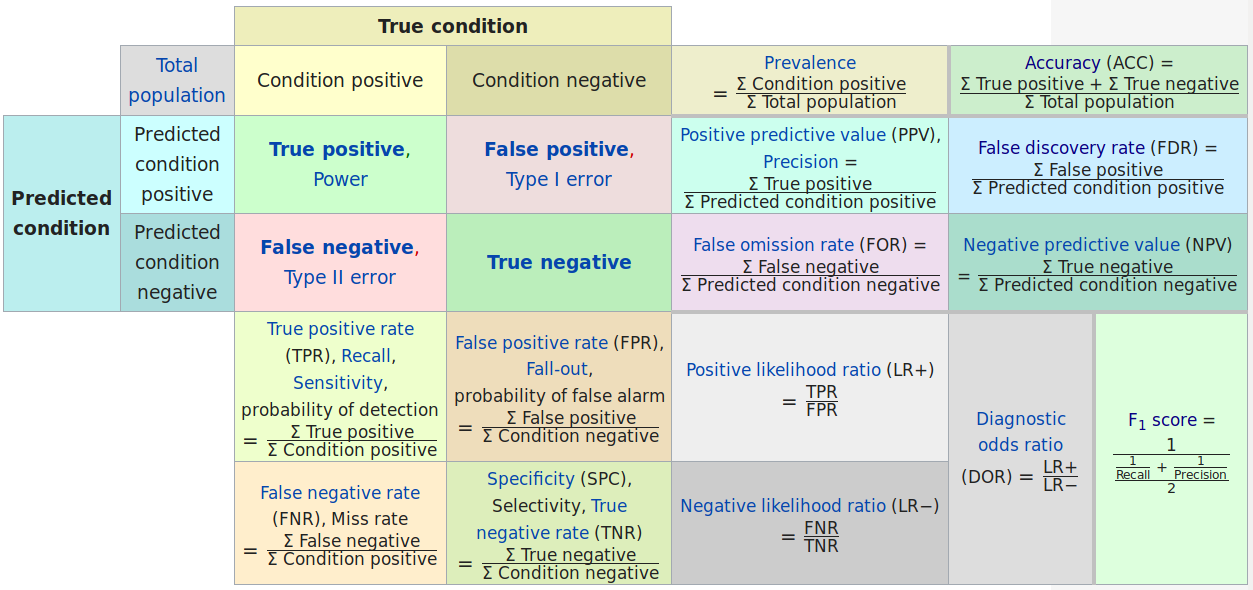
\includegraphics[width=\textwidth]{evaluation_methods_binary_classification.png}
	%\caption{Image taken with a non-mydriatic fundus camera.}
\end{figure}
\tiny Source: \url{https://en.wikipedia.org/wiki/Sensitivity_and_specificity}
\end{frame}

\begin{frame}{Evaluation Measures}{Inter-rater agreement}
\begin{itemize}
	\item Used for measuring agreement between raters
	\item Kappa (binary classification, no gold standard) $\quad \kappa = \frac{P_0 - P_e}{1 - P_e}$
	\item Weighted Kappa (ordinal categories, penalization grows with distance) $\quad \kappa_w = \frac{\sum_{i,j} \omega_{i,j}O_{i,j}}{\sum_{i,j} \omega_{i,j} E_{i,j}}$
	\item Intra-class correlation (when outcome measured on a continous scale)
\end{itemize}

\begin{table}
	\caption{Table for interpretation of Weighted Kappa, after Landis \& Koch (1977)}	
	\centering
	\begin{tabular}{llr}
		\hline
		$\kappa$    & Strength of agreement \\
		\hline
		$\leq 0.20$ 	& Poor \\
		$0.21-0.40$ 	& Fair \\
		$0.41-0.60$ 	& Moderate \\
		$0.61-0.80$ 	& Good \\
		$0.81-1.00$ 	& Very good \\
		\hline
	\end{tabular}
\end{table}
\end{frame}

\subsection{Machine Learning}

\subsection{Methods}

\begin{frame}{Methods Used in this thesis}{}
\begin{columns}
	\begin{column}{0.5\textwidth}

\begin{figure}[!h]
	\centering
	\scalebox{0.4}{
		\smartdiagramset{
			distance text center bubble=0.5cm,
			bubble center node size=3cm,
			bubble node size=3cm,
			distance center/other bubbles=2.5cm,
			bubble center node font=\LARGE,
			bubble node font=\LARGE,
			bubble center node color=magenta,
			set color list = {yellow, pink, blue, green, black}
		}%		
		\smartdiagram[bubble diagram:vertical]{
			Machine\\Learning, 
			Supervised\\Learning, 
			Image\\Classification, 
			Convolutional\\Neural\\Networks,
			Ensembling\\Techniques
		}
	}
	%\caption{Traditional pattern recognition scheme}
\end{figure}

	\end{column}
	\begin{column}{0.5\textwidth}
\alert{Traditional pattern recognition scheme:}		
\begin{figure}[!h]
	\centering
	\smartdiagramset{back arrow disabled=true}
	\resizebox{.9\linewidth}{!}{\smartdiagram[flow diagram:horizontal]{Image Input, Hand-Crafted Feature Extractor, 'Simple'\\Classifier, Class}}
	%\label{back:fig:trad_pat_rec}
\end{figure}
\alert{Deep Learning pattern recognition scheme (end-to-end learning):}
\begin{figure}[!h]
	\centering
	\smartdiagramset{back arrow disabled=true}
	\resizebox{.9\linewidth}{!}{\smartdiagram[flow diagram:horizontal]{Image Input, Trainable Feature Extractor, Trainable Classifier, Class}}
	%\label{back:fig:dl_pat_rec}
\end{figure}

	\end{column}
\end{columns}
\end{frame}

\subsection{Data}

\begin{frame}{The dataset: EyePACS}{Whole dataset of near 88,692 images, 10x10}
\includegraphics[width=1.0\textwidth]{mosaic-85000-10x10.png}	
\end{frame}

\begin{frame}{The dataset: EyePACS}{10,000 random images, 25x25}
\includegraphics[width=1.0\textwidth]{mosaic-10000-25x25.png}	
\end{frame}

\begin{frame}{The dataset: EyePACS}{2,000 random images, 50x50}
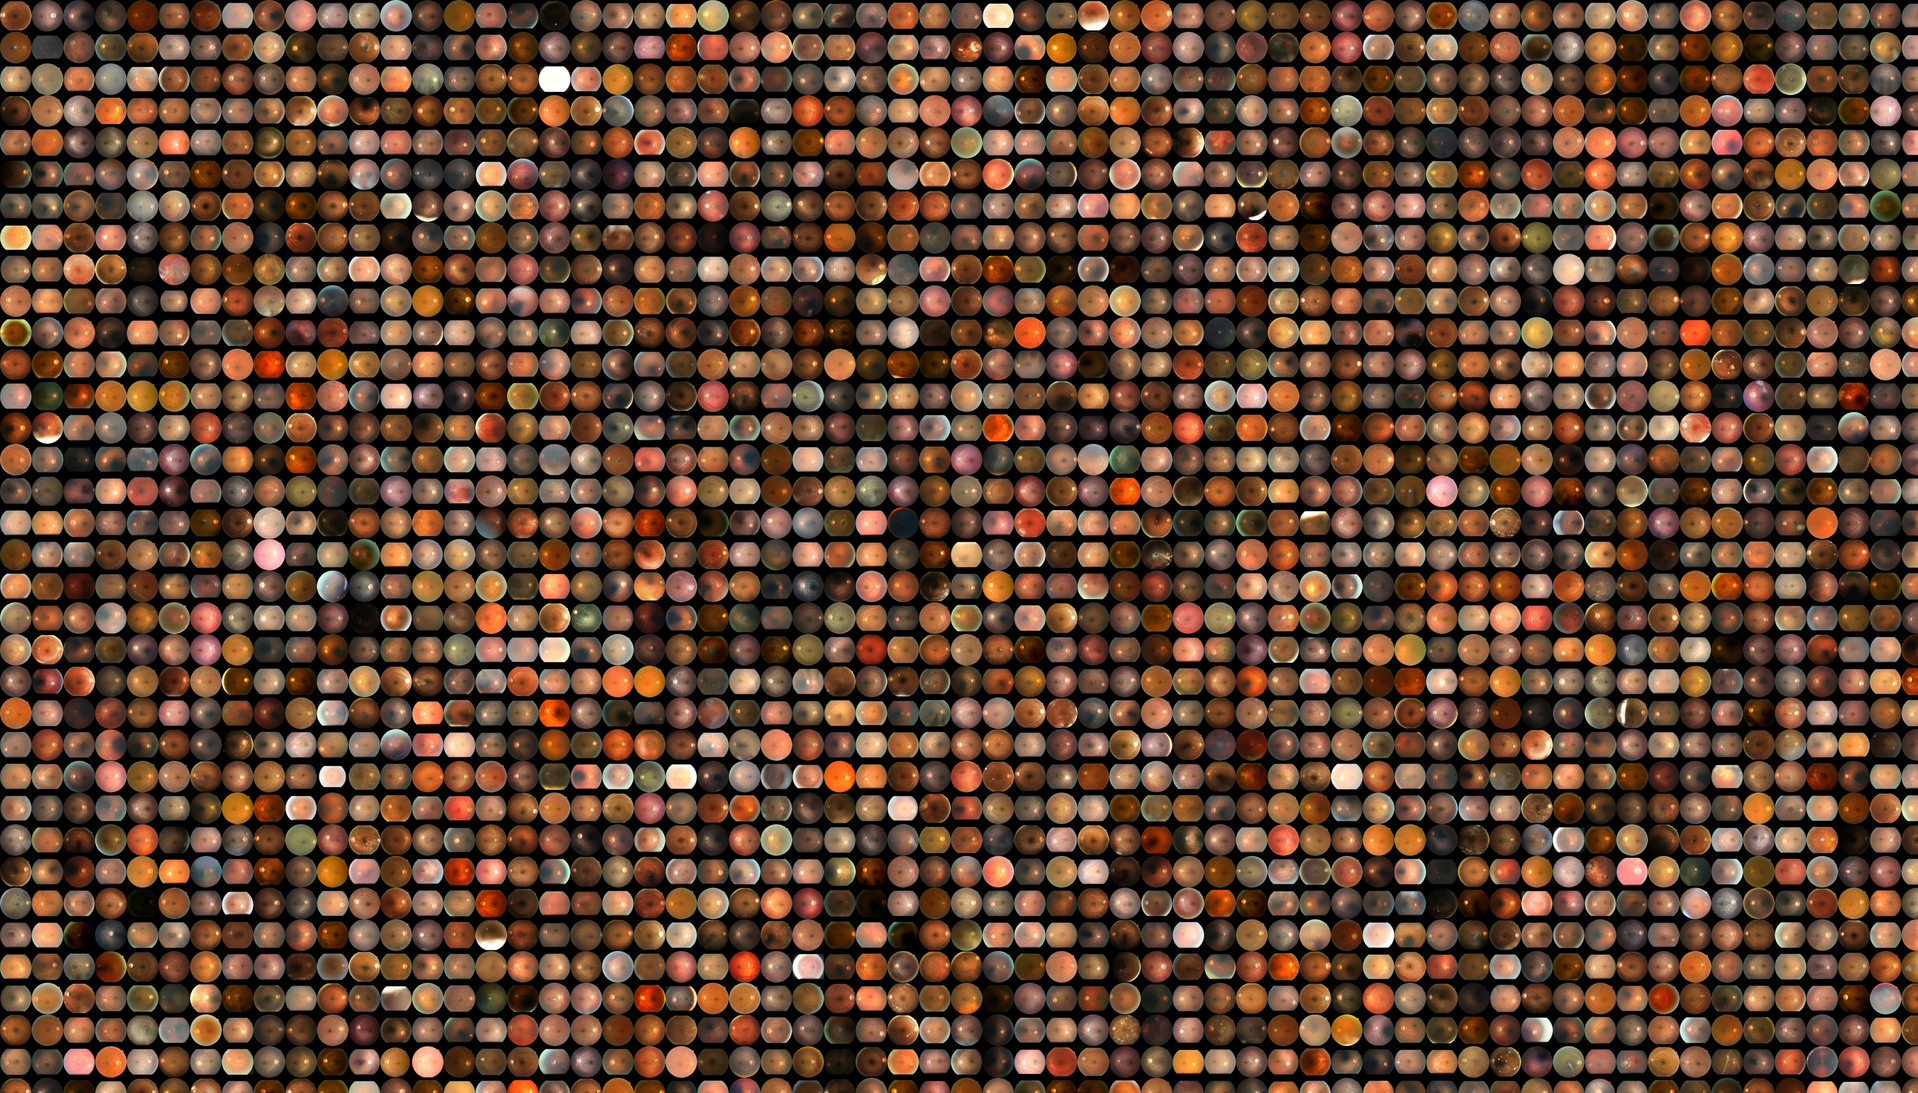
\includegraphics[width=1.0\textwidth]{mosaic-2000-50x50.png}	
\end{frame}

\begin{frame}{The dataset: EyePACS}{500 random images, 100x100}
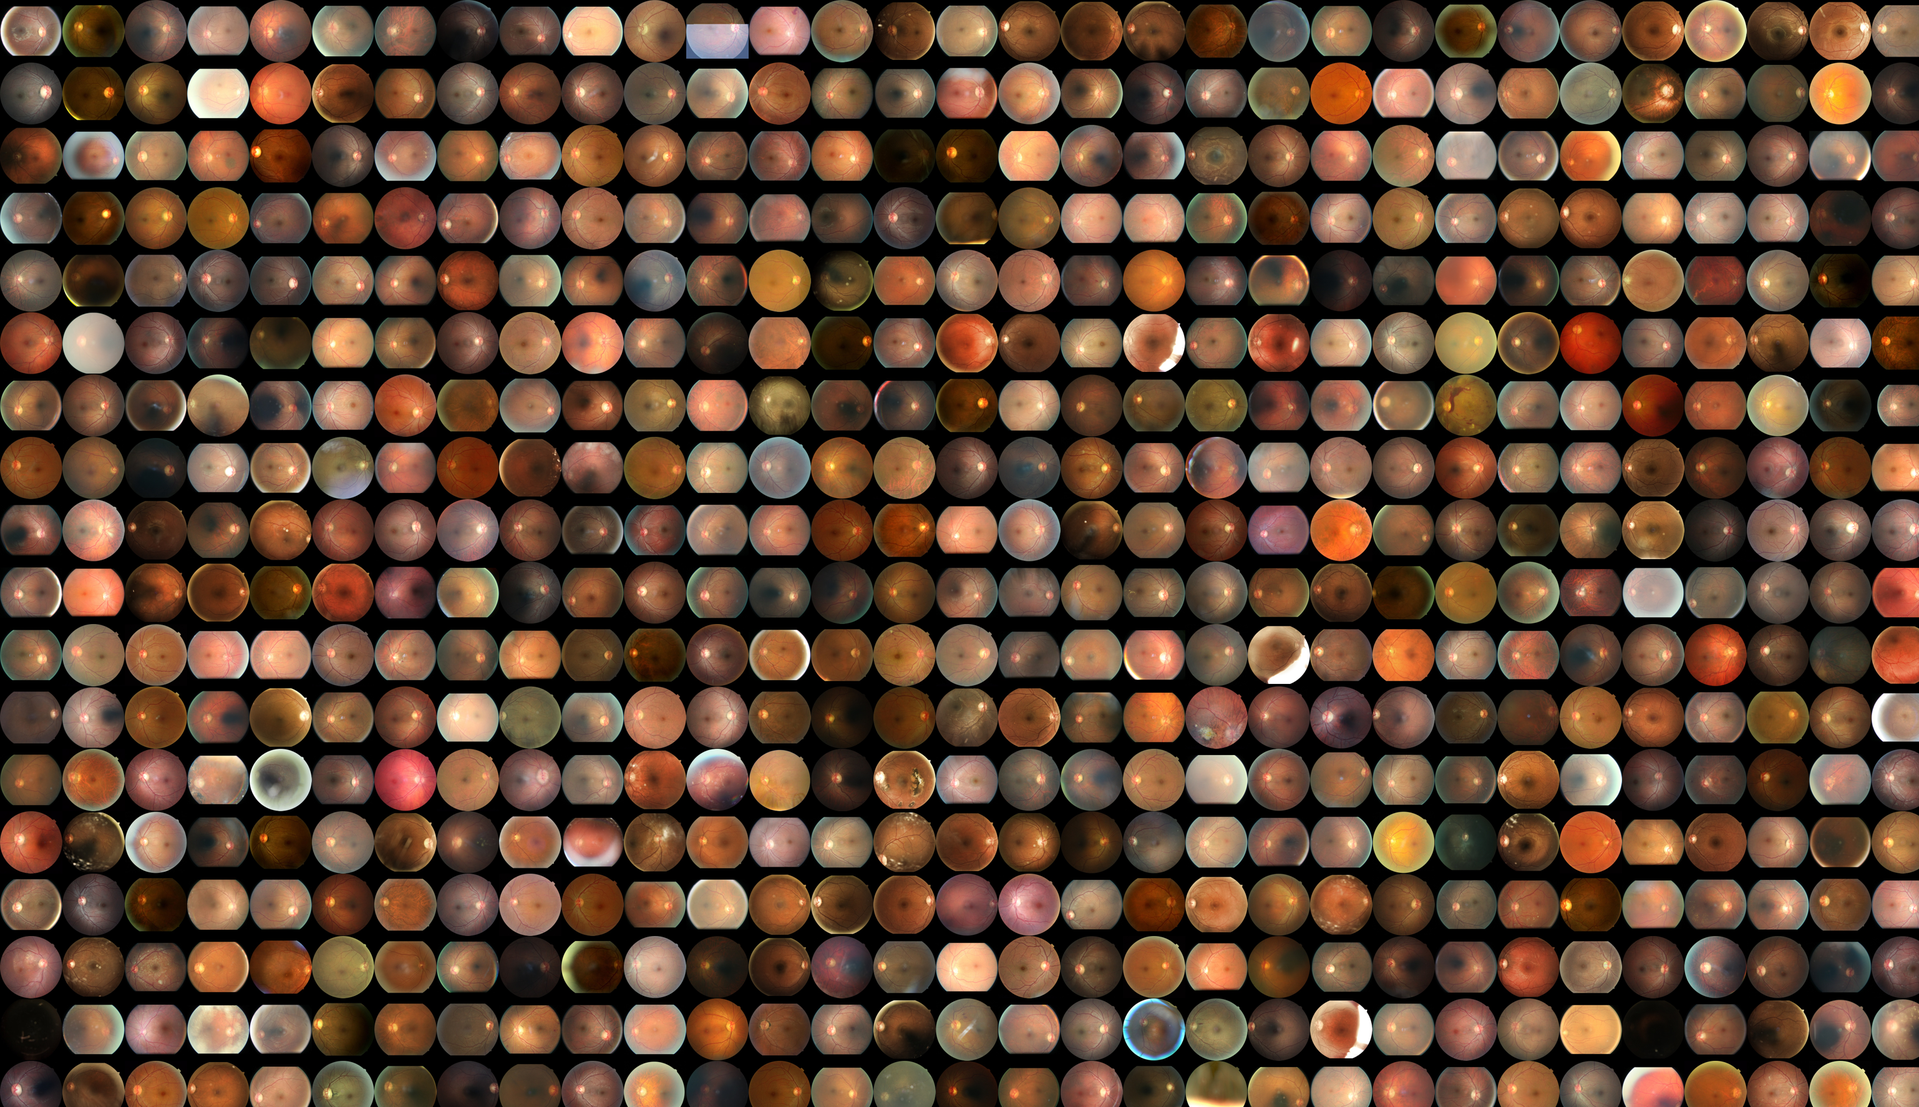
\includegraphics[width=1.0\textwidth]{mosaic-500-100x100.png}	
\end{frame}


\begin{frame}{EyePACS dataset}{}
%\begin{columns}
%\begin{column}{0.5\textwidth}
%\begin{figure}[p]
%\resizebox{.61\textwidth}{!}{
%\begin{tikzpicture}[scale = 0.95]
%\pie[sum=auto , after  number=, radius = 2.5, explode={0, 0, 0.1}]{31.613/Train, 3.513/Validation,  53.576/Test}
%\end{tikzpicture}
%}
%\caption{Dataset conformation}
%\end{figure}	
%\end{column}
%\begin{column}{0.4\textwidth}  %%<--- here
\begin{figure}[p]
\resizebox{.60\textwidth}{!}{
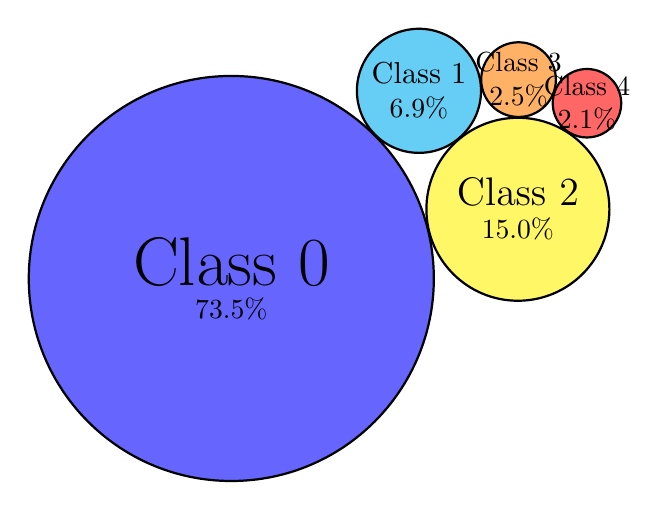
\begin{tikzpicture}[scale=0.10]
\pie[cloud, text=inside,scale font, radius=30]
{
	73.5/Class 0,
	6.9/Class 1,
	15.0/Class 2,
	2.5/Class 3,
	2.1/Class 4
}
\end{tikzpicture}
}
%\caption{Dataset class percentage}
\end{figure}
%\end{column}
%\end{columns}	
\begin{itemize}
\item $88,692$ retina fundus images of differing sizes, illumination conditions, quality.\\ 
\item  $44,346$ different patients. For every patient: right and left eye images available.
\end{itemize}
\end{frame}

\begin{frame}{The dataset}{Minimal data pre-processing}
Minimal data preprocessing applied (optimization of hardware resources, deep learning optimization methods are computer intensive tasks): 
\begin{itemize}
\item Remove borders
\item Standardization of the image size (downsizing: 128, 256, 512, etc.) depending on the model requirements.
\end{itemize}

\begin{columns}
\begin{column}{0.5\textwidth}
\begin{figure}[p]
\resizebox{.74\textwidth}{!}{
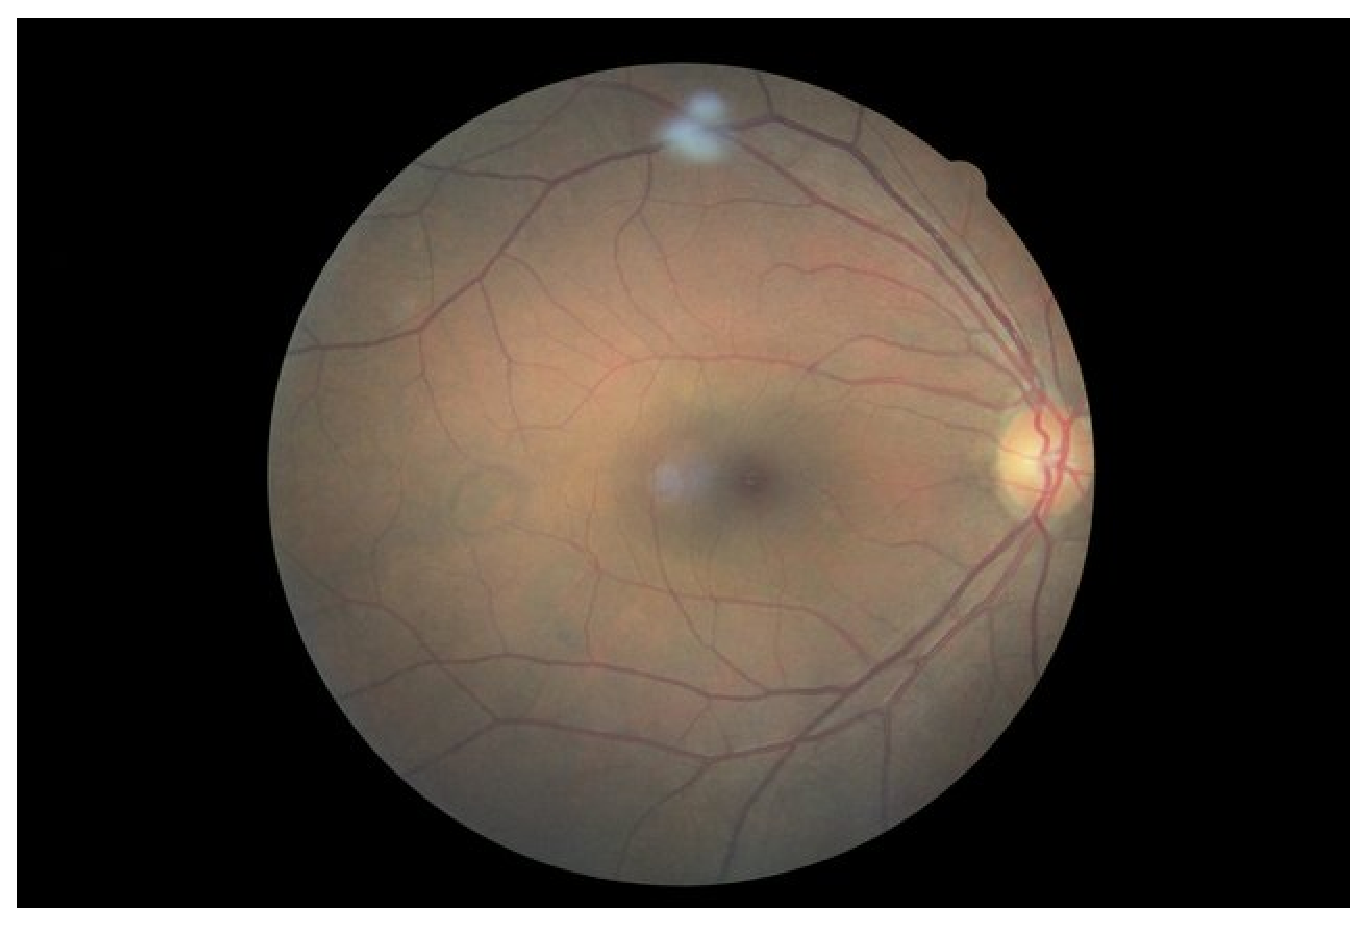
\includegraphics[width=1.0\textwidth]{61_right-4752x3168.eps}
}
\caption{Original 4752x3168 pixels}
\end{figure}	
\end{column}
\begin{column}{0.31\textwidth}  %%<--- here
\begin{figure}[p]
\resizebox{.74\textwidth}{!}{
\includegraphics[width=1.0\textwidth]{61_right-4752x3168-trimmed.eps}
}
\caption{Preprocessed: trimmed + resized}
\end{figure}
\end{column}
\end{columns}	
\end{frame}


\part{Classification}

\section{Preliminary Models}

%\subsection{Mathematical formalization}
% You can reveal the parts of a slide one at a time
% with the \pause command:
\begin{frame}{Classification - Preliminary models}{Mathematical formalization of the classification problem}
\begin{itemize}
	\item {   
		Find a function f: $\mathbb{R}^{CxHxW} 
		\mapsto \mathbb{R}^{n}$ that maximizes a objective function (where $CxHxW \gg n$). \alert{Optimization}.
	}
	% You can also specify when the content should appear
	% by using <n->:
	\item {
		Images are high dimensional objects with highly correlated local points.
		Function proven to exploit these characteristics: a \alert{deep convolutional neural network}.
	}
	\item {
		\alert{Objective function} in neural network argot called \alert{cost function}.
	}
	% or you can use the \uncover command to reveal general
	% content (not just \items):
	\item {
		Standardized cost function for classification: \alert{logarithmic loss} (log-loss).
	}
	\item {
		Evaluation metric: \alert{quadratic weighed kappa} (QWK).
	}
\end{itemize}
\end{frame}

\begin{frame}{Classification - Preliminary models}{Preliminary Models - Key points of this work}
\begin{columns}
	\begin{column}{0.7\textwidth}
		\begin{itemize}
			\item Data augmentation techniques were necessary to balance the classes and to increment the generalization capabilities of the model (brightness,contrast, rotations).
			\item Due to hardware limitations only a part of the input was feeded to the network (about 71\% of the useful information), requiring various evaluations and ensembling on test time to increase performance.
			\item Probabilistic combination of results of both eyes (Bayes rule) helps improve further performance. (Thesis contribution)
		\end{itemize}
	\end{column}
	\begin{column}{0.3\textwidth}
		\begin{figure}[p]
			\resizebox{.75\textwidth}{!}{
				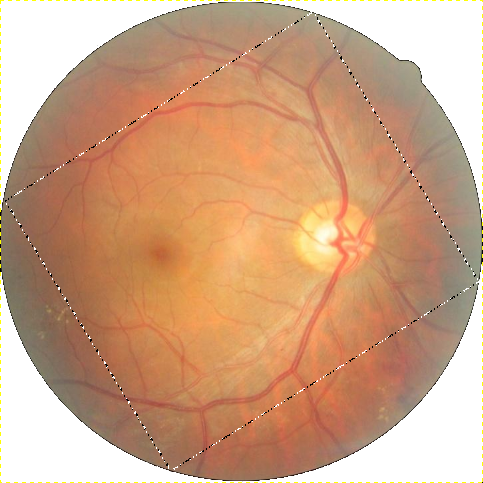
\includegraphics[width=1.0\textwidth]{input-ccia2016-paper.png}
			}
			\caption{Input data selection}
		\end{figure}
	\end{column}
\end{columns}
\end{frame}

\begin{frame}{Classification - Preliminary models}{Preliminary models - Model and training overview (CCIA 2016)}	
\begin{columns}
\begin{column}{0.2\textwidth}
	\centering
	\alert{Model}
	\begin{figure}[p]
		\resizebox{.5\textwidth}{!}{
			\includegraphics[width=1.0\textwidth]{nnarch-crop.pdf}	
		}
		%\caption{Model}
	\end{figure}
\end{column}
\begin{column}{0.4\textwidth}
	\centering
	\alert{Training}
	\begin{figure}[p]
		\resizebox{.4\textwidth}{!}{
			\includegraphics[width=1.0\textwidth]{training-crop.pdf}
		}
		%\caption{Training}
	\end{figure}	
\end{column}
\begin{column}{0.4\textwidth}  %%<--- here
	\alert{Evaluation}
	\begin{figure}[p]
		\resizebox{0.9\textwidth}{!}{
			\includegraphics[width=\textwidth]{testing-crop.pdf}				
		}
		%\caption{Evaluation}
	\end{figure}
	\alert{Combination}
	\begin{figure}[p]
		\resizebox{\textwidth}{!}{
			\includegraphics[width=\textwidth]{combination-crop.pdf}	
		}
		%\caption{Combination}
	\end{figure}
\end{column}
\end{columns}	
\end{frame}

\begin{frame}{Classification - Preliminary models}{Preliminary models - Results}	
\begin{table}[h!]
\centering
\begin{tabular}{c c c c} 
\hline		
Layers & Input size & $\kappa_{test, alone}$ & $\kappa_{test, combined}$\\ [0.5ex] 
\hline\hline
12 & (3,128,128) & 0.488 & 0.577\\ 
14 & (3,256,256) & 0.636 & 0.660\\ 
16 & (3,384,384) & 0.668 & 0.730 \\ 
16 & (3,512,512) & 0.725 & 0.769\\ 
\hline
\end{tabular}
\caption{Comparison of results obtained with and without probabilistic combination}
\label{table-results2}
\end{table}
\end{frame}


\begin{frame}{Classification - Preliminary models}{Summary of the methods used}
\begin{itemize}
	\item Data augmentation techniques
	\item Stochastic Gradient Descent
	\item Logarithmic loss function
	\item Partial input information due to hardware limitations
	\item Ensembling techniques with different versions of the same image (geometric mean of 5 different evaluations)
	\item Ensembling techniques for combination of the information of both eyes (Bayes rule)
\end{itemize}	
\end{frame}

\section{QWK loss function for ordinal regression}

\begin{frame}{QWK: A new loss function for ordinal regression}{Mathematical summary of the paper (Pattern Recognition Letters, 2017)}	
Model function: $p = f(I) \quad where \quad I \in \mathbb{R}^{CxHxW}, \quad p \in \mathbb{R}^n$
\begin{columns}
	\begin{column}{0.5\textwidth}
		\\
		\alert{Log-loss optimization:}
		\begin{equation*}
		min \quad C = \sum_{i=1}^{BS} \sum_{j=1}^{n} t_{i,j} log(p_{i,j})
		\end{equation*}			
		First order derivative:\\
		\begin{equation*}
		\frac{\partial C}{\partial p_{i,j}} = \frac{t_{i,j}}{p_{i,j}}
		\end{equation*}							
	\end{column}
	\begin{column}{0.5\textwidth}  %%<--- here
		\\
		\alert{QWK-loss optimization:}\\
		\begin{equation*}
		max \quad \kappa = \frac{\sum_{i,j} \omega_{i,j}O_{i,j}}{\sum_{i,j} \omega_{i,j} E_{i,j}} 
		\end{equation*}		
		\begin{equation*}
		min \quad C = log(1 - \kappa), \quad \omega_{i,j} = \frac{(i-j)^2}{(n-1)^2}
		\end{equation*}		
		First order derivative: (next slide)			
	\end{column}
\end{columns}	
\end{frame}

\begin{frame}{QWK: A new loss function for ordinal regression}{Mathematical summary of the paper (Pattern Recognition Letters, 2017)}	
\alert{QWK first order derivative:}
\begin{columns}
	\begin{column}{0.3\textwidth}
		\begin{equation*}
		\frac{\partial \mathcal{L}}{\partial y_m} = \frac{1}{\mathcal{N}}\frac{\partial \mathcal{N}}{\partial y_m} - \frac{1}{\mathcal{D}}
		\frac{\partial{\mathcal{D}}}{\partial y_m}
		\end{equation*}	
		
		where:
		
		\begin{equation*}
		\frac{\partial \mathcal{N}}{\partial y_m(X_k)} = \omega_{t_k m}
		\end{equation*}
		
		\begin{equation*}
		\frac{\partial \mathcal{D}}{\partial y_m(X_k)} = \sum_{i=1}^{C} \hat{N_i} \omega_{i,m}
		\end{equation*}
		
		\begin{itemize}
			\item[] $m \in \{1, 2, ..., C\}$
		\end{itemize}
		
	\end{column}
	\begin{column}{0.7\textwidth}  %%<--- here
		\begin{equation*}
		\begin{aligned}
		\frac{\partial \mathcal{N}}{\partial y_m} =
		\begin{pmatrix} 
		\omega_{t_1, 1}     & \omega_{t_1, 2}     & ...     & ... & \omega_{t_1, C}\\ 
		\omega_{t_2, 1}     & \omega_{t_2, 2}     & ...     & ... & \omega_{t_2, C}\\ 
		...					& ...		          & ...     & ... & ...\\
		\omega_{t_N, 1}     & \omega_{t_N, 2}     & ...     & ... & \omega_{t_N, C}\\  
		\end{pmatrix}
		\end{aligned}
		\end{equation*}
		
		\begin{equation*}
		\begin{aligned}
		\frac{\partial \mathcal{D}}{\partial y_m} =
		\begin{pmatrix} 
		\sum_{i=1}^C \hat{N_i} \omega_{1,i} & ...  & ...     & ... & \sum_{i=1}^C \hat{N_i} \omega_{C,i}\\
		\sum_{i=1}^C \hat{N_i} \omega_{1,i} & ...  & ...     & ... & \sum_{i=1}^C \hat{N_i} \omega_{C,i}\\
		... & ::: & ... & ... & ...\\
		\sum_{i=1}^C \hat{N_i} \omega_{1,i} & ...  & ...     & ... & \sum_{i=1}^C \hat{N_i} \omega_{C,i}\\ 
		\end{pmatrix}
		\end{aligned}
		\end{equation*}	
	\end{column}
\end{columns}	
\end{frame}


\begin{frame}{QWK: A new loss function for ordinal regression}{Pattern Recognition Letters, 2017}	
\begin{itemize}
\item  Three different multi-class classification problems using as evaluation metric QWK were trained using QWK-loss and log-loss.
\item Different neural networks were tested: a linear classifier, a shallow neural network of 2-3 layers and a deep neural network of up to 16 layers.
\item Optimizing QWK reported in all the models and problems increases of performance in the test set of about 5 to 10\% over the conventional training method.
\end{itemize}	
\end{frame}

\begin{frame}{QWK: A new loss function for ordinal regression}{Results for "Search Results Relevance" Case Study}	
\begin{figure}[p]
	\resizebox{\textwidth}{!}{
		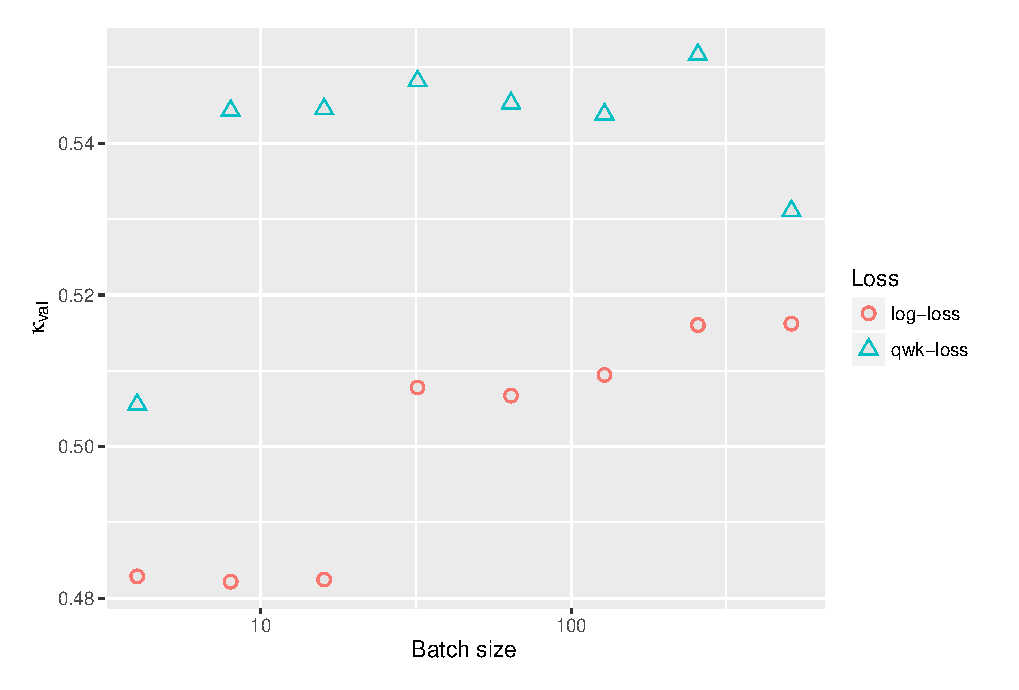
\includegraphics[width=1.0\textwidth]{crowdflower-results.eps}
	}
	%\caption{LC for search results relevance}
\end{figure}
\end{frame}

\begin{frame}{QWK: A new loss function for ordinal regression}{Results for "SNN Insurance Assessment" Case Study}	
\begin{figure}[p]
	\resizebox{\textwidth}{!}{
		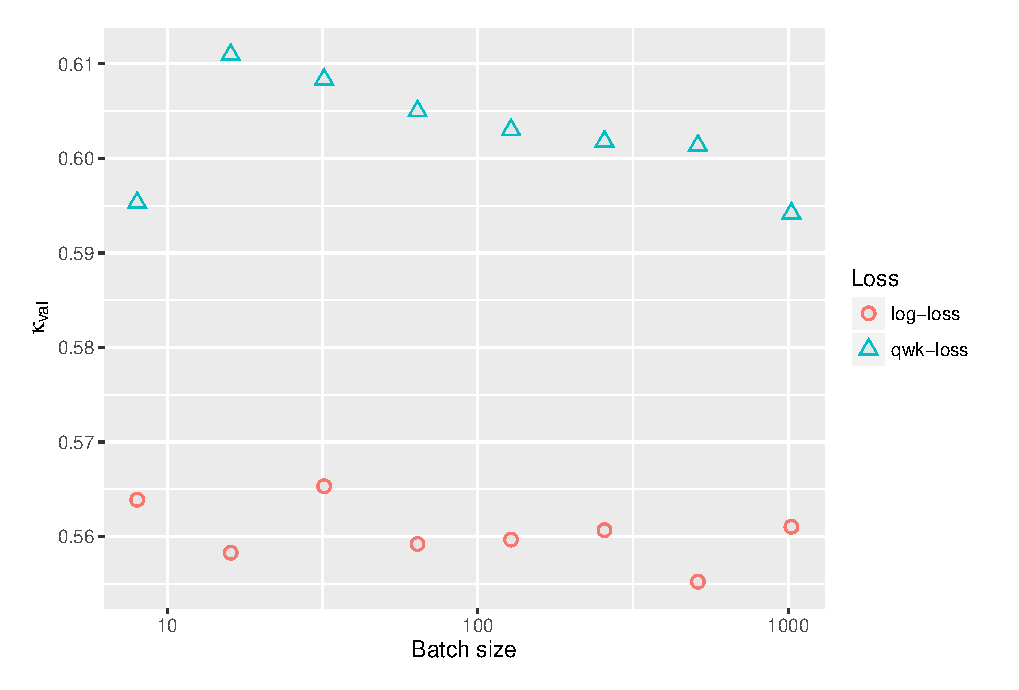
\includegraphics[width=1.0\textwidth]{prudential-results.eps}
	}
	%\caption{LC for search results relevance}
\end{figure}
\end{frame}

\begin{frame}{QWK: A new loss function for ordinal regression}{Results for "Diabetic Retinopathy Disease Grading" Case Study}	
\begin{figure}[p]
	\resizebox{\textwidth}{!}{
		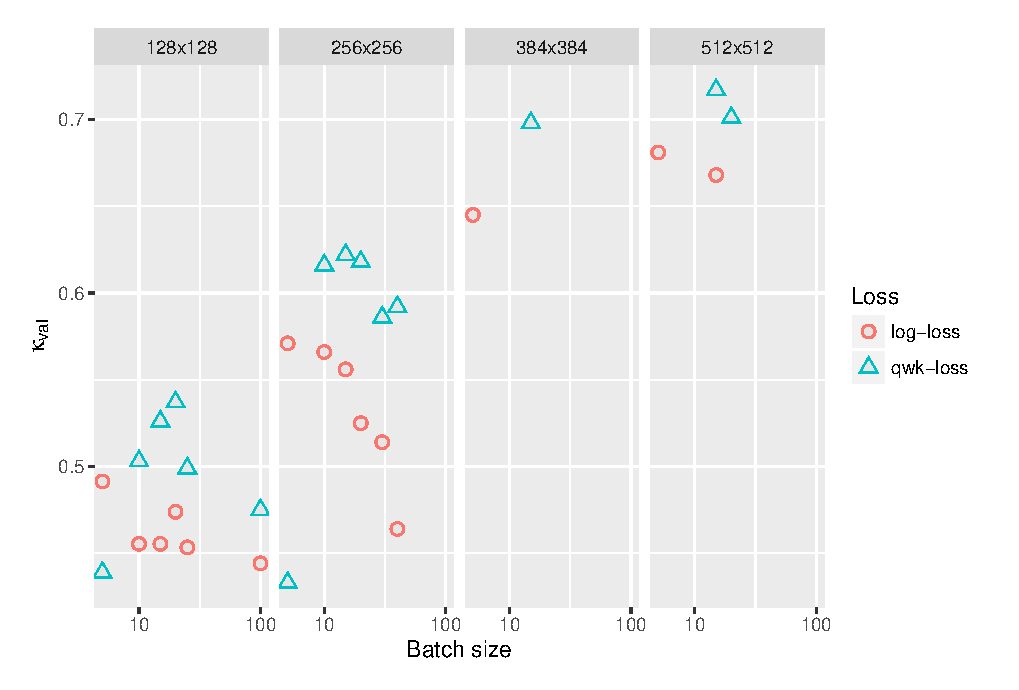
\includegraphics[width=1.0\textwidth]{retine-results.eps}
	}
	%\caption{LC for search results relevance}
\end{figure}
\end{frame}

\begin{frame}{QWK: A new loss function for ordinal regression}{Test set confidence intervals for each case study}	
\begin{figure}[p]
	\resizebox{0.85\textwidth}{!}{
		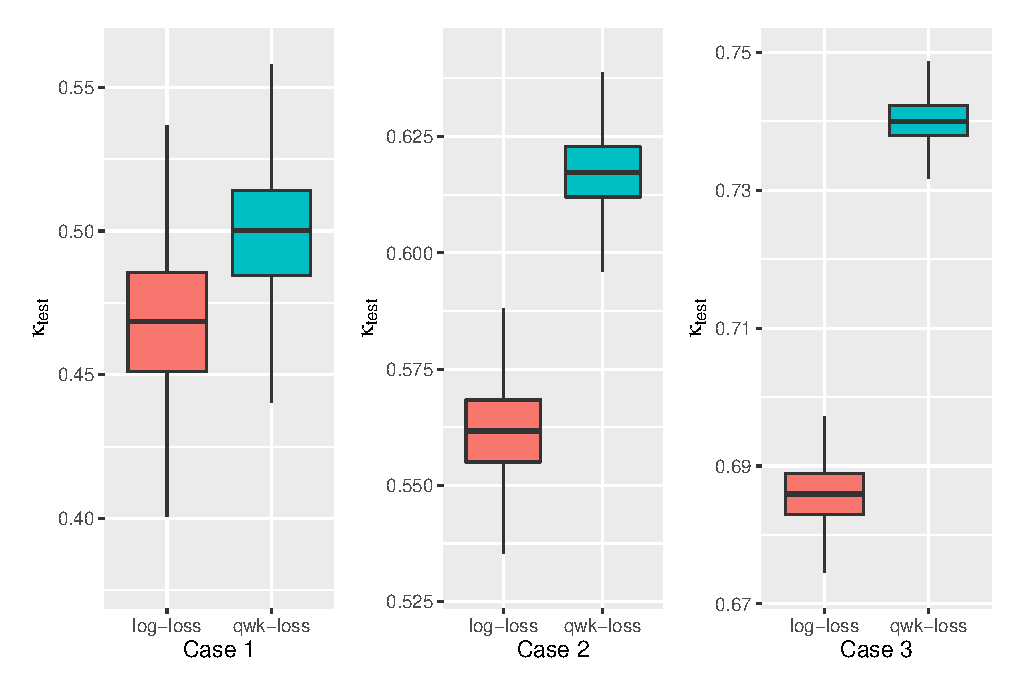
\includegraphics[width=\textwidth]{boxplots.eps}
	}
	%\caption{LC for search results relevance}
\end{figure}
\end{frame}

\section{Enhanced models}

\begin{frame}{Classification - Enhanced Models}{Guidelines}
\begin{itemize}
	\item Use an optimal image resolution \\Tested 128, 256, 384, 512, 640, 724, 768, 892. Optimal: 640
	\item Use all available information
	\item Use a fully convolutional neural network
	\item Use small size convolutions \\Feature extraction 3x3 and 2x2 in classification layer
	\item Adapt convolution sizes and number of layers to get a RF as close as possible to the image size
	\item Use ReLU as activation function
	\item Use batch normalization in every layer
	\item Use QWK as loss function
	\item Use a linear classifier
	\item Use an efficient number of features \\Tested: 32 to 512. Optimal: 64
\end{itemize}
\end{frame}

\begin{frame}{Classification - Enhanced Models}{Design}
Prediction model of 391,325 trainable parameters located in blue blocks.	
\begin{columns}
	\begin{column}{0.2\textwidth}  %%<--- here		
		\begin{figure}[p]
			\resizebox{.6\textwidth}{!}{
				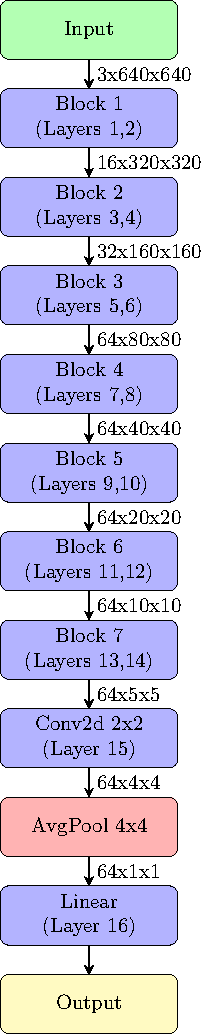
\includegraphics[width=1.0\textwidth]{model640.pdf}				
			}
			%\caption{Best prediction model}
		\end{figure}		
	\end{column}
	\begin{column}{0.2\textwidth}  %%<--- here		
	\begin{figure}[p]
		\resizebox{.7\textwidth}{!}{
			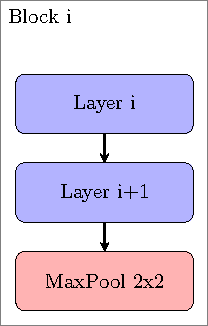
\includegraphics[width=1.0\textwidth]{modelblock.pdf}		
		}
		%\caption{Best prediction model}
	\end{figure}
	\begin{figure}[p]
	\resizebox{.6\textwidth}{!}{
		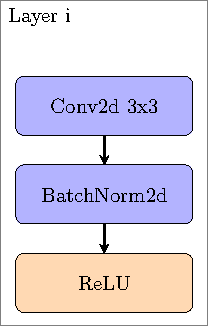
\includegraphics[width=1.0\textwidth]{modellayer.pdf}		
	}
	%\caption{Best prediction model}
	\end{figure}
		
	\end{column}
	\begin{column}{0.55\textwidth}
	\begin{figure}[p]
	\resizebox{.55\textwidth}{!}{
		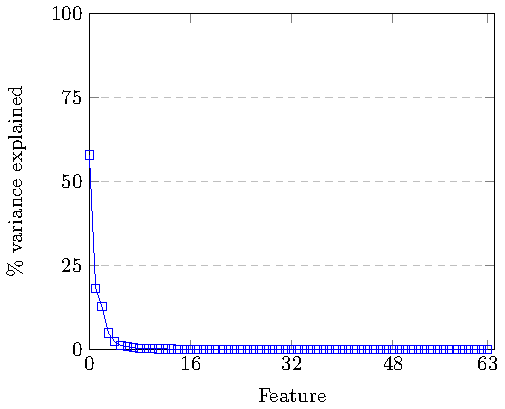
\includegraphics[width=1.0\textwidth]{PCA_feature_space.pdf}		
	}
	%\caption{Best prediction model}
	\end{figure}	
	\begin{figure}[p]
	\resizebox{.55\textwidth}{!}{
		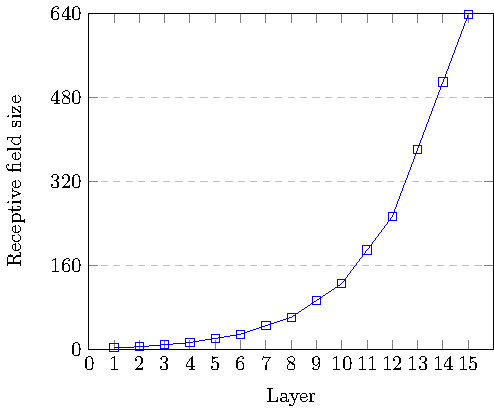
\includegraphics[width=1.0\textwidth]{receptive_field_640.pdf}		
	}
	%\caption{Best prediction model}
	\end{figure}	
	\end{column}
\end{columns}	
\end{frame}

\begin{frame}{Classification - Enhanced Models}{Results: EyePACS Dataset over a test set of $10,000$ images of $5,000$ different patients}	

Inter-rater agreement 5 classes:
\begin{itemize}
	\item $QWK=0.801$ with information of one eye
	\item $QWK=0.844$ with information of both eyes \\(same feature extractor, retrained last linear layer)
\end{itemize}
Group detection of the most severe cases of DR \\(classes 2, 3 and 4): 
\begin{itemize}
	\item Sensitivity=$0.906$ ($95$\% CI: $0.893$ to $0.919$)
	\item Specificity=$0.847$ ($95$\% CI: $0.840$-$0.855$)
	\item Accuracy=$0.857$
	\item $F_1$ = $0.710$
	\item MCC=$0.648$
\end{itemize}
\end{frame}

\begin{frame}{Classification - Enhanced Models}{Results: Messidor-2 Dataset over a test set of $1,748$ images}	

Inter-rater agreement 4 classes:
\begin{itemize}
	\item $QWK=0.830$ with information of one eye
\end{itemize}
Group detection of the most severe cases of DR \\(classes 2, 3): 
\begin{itemize}
	\item Sensitivity=$0.908$ ($95$\% CI: $0.883$-$0.933$)
	\item Specificity=$0.911$ (95\% CI: $0.890$-$0.933$)
	\item Accuracy=$0.910$
	\item $F_1$ = $0.896$
	\item MCC=$0.817$
\end{itemize}
\end{frame}

\begin{frame}{Classification - Enhanced Models}{Results: Classification Benchmarks over Messidor-2 Dataset}	


\begin{table}[ht]
	\centering
	\scalebox{1.0}{
		\begin{tabular}{crrrr}
			\hline
			Reference & Parameters & Depth & Sensitivity & Specificity\\ \hline
			(Gulshan et al., 2016) & $23,851,784$ & 159 & 96.1 \% & 93.9 \% \\ 
			Our work & $391,325$ & 17 & 91.1 \% & 90.8 \% \\
			\hline	
		\end{tabular}
	}
	\caption{Prediction performance \& model complexity comparison of our proposal vs the state-of-the-art model (Messidor-2 data set)}
	\label{class2:tab:bench} 
\end{table}
\begin{itemize}
	\item Our model differentiate between the five disease classes, detecting also the milder cases (of medical interest for early detection).
	\item (Gulshan et al., 2016) is a binary classifier specialized in detection of the most severe cases of the disease
\end{itemize}
\end{frame}

\section{Classification model stability}

\begin{frame}{Classification Model Stability}{}	

\begin{itemize}
	\item Deep learning models have a huge parameter set (millions of parameters), ie. are difficult to analyze
	\item Model validity is tested against a test set ideally coming from the same data distribution, having a statistical information about its general behavior
	\item For a better understanding of model capabilities and limitations a study of variation of outputs vs variations in inputs is proposed.
	\item Proposed variables of study: rotation, hue, saturation and lightness
\end{itemize}
\end{frame}

\begin{frame}{Classification Model Stability}{Variables of study: rotation, hue, saturation and lightness}
\begin{columns}
	\begin{column}{0.6\textwidth}
		\begin{itemize}
			\item Rotation
			\item Hue referring to
			the attribute of a visual sensation according to which an area appears to be similar to one of the perceived colors: red, yellow, green, and blue, or to a
			combination of two of them 
			\item Lightness representing the brightness relative to the brightness of a similarly illuminated white
			\item Saturation showing the colorfulness of a
			stimulus relative to its own brightness
		\end{itemize}	
	\end{column}
	\begin{column}{0.4\textwidth}  %%<--- here
		\begin{figure}[p]
			\centering
			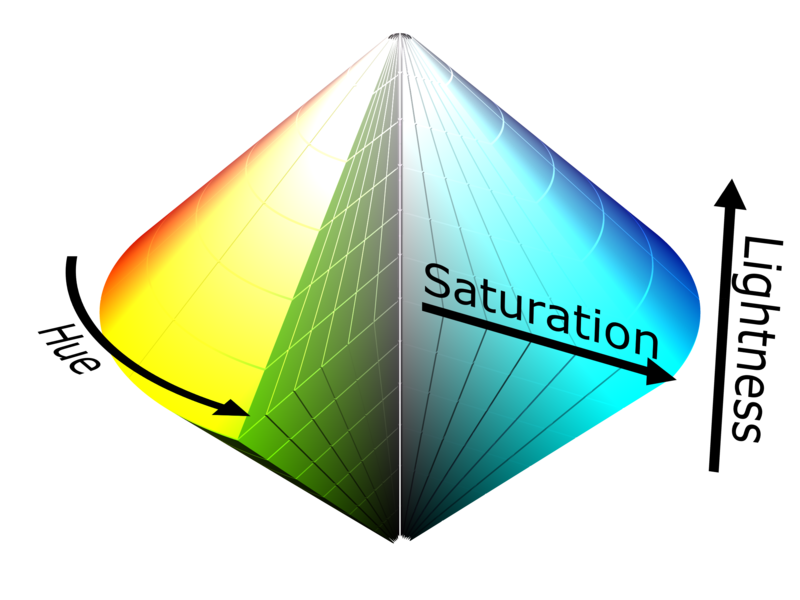
\includegraphics[width=\textwidth]{HSL_color_solid_dblcone.png}
			\caption{HSL color space}
		\end{figure}
	\end{column}
\end{columns}

\end{frame}

\begin{frame}{Stability analysis sample}{20060412 61593 0200 PP Target: 1 HSL}
\begin{columns}
\begin{column}{0.3\textwidth}
\begin{figure}[p]
\centering
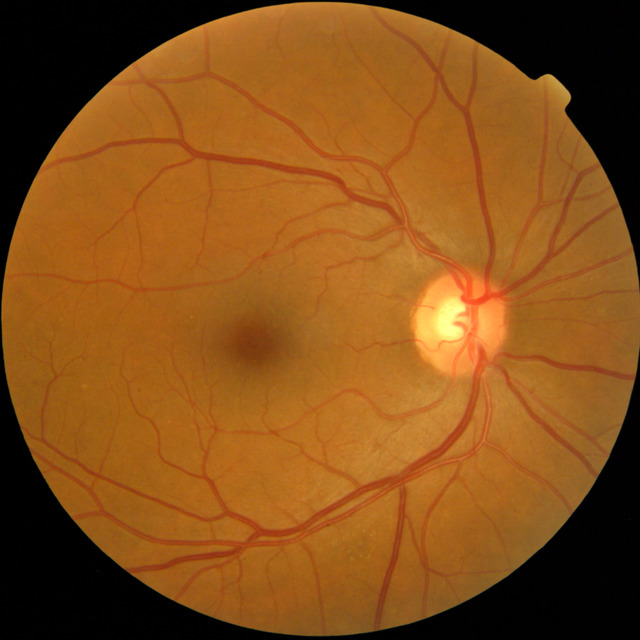
\includegraphics[width=\textwidth]{chapter_stability/20060412_61593_0200_PP/20060412_61593_0200_PP.jpeg}
%\caption{}
\end{figure}	
\end{column}
\begin{column}{0.45\textwidth}  %%<--- here
\begin{figure}[p]
\centering
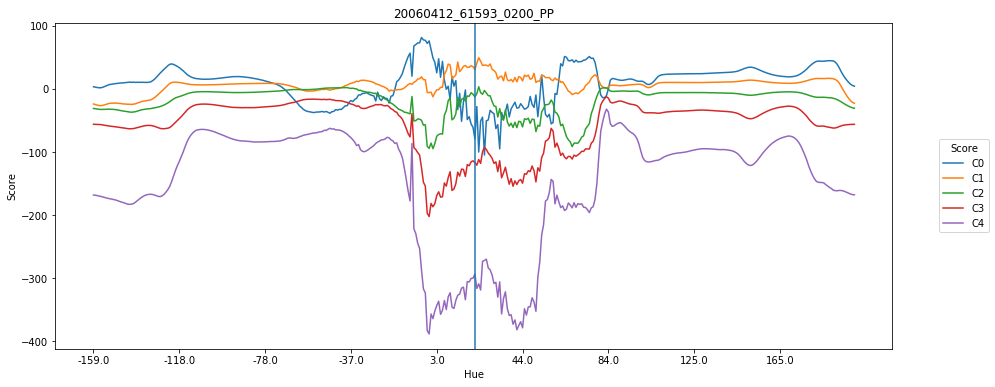
\includegraphics[width=\textwidth]{chapter_stability/20060412_61593_0200_PP/h/scores.png}			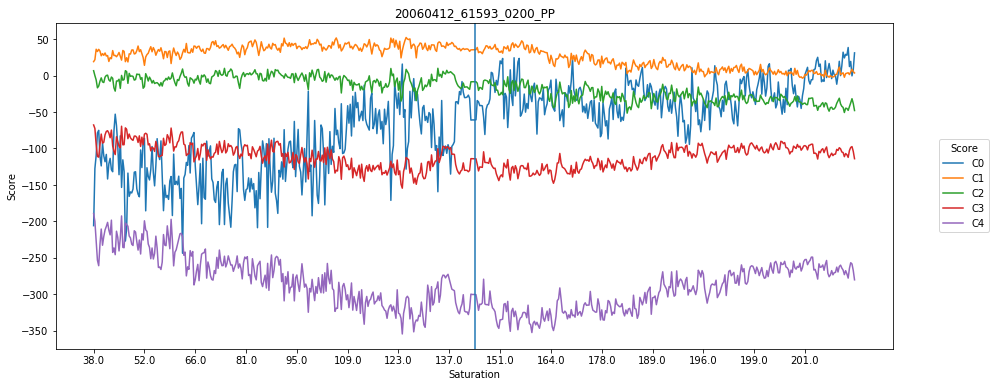
\includegraphics[width=\textwidth]{chapter_stability/20060412_61593_0200_PP/s/scores.png}			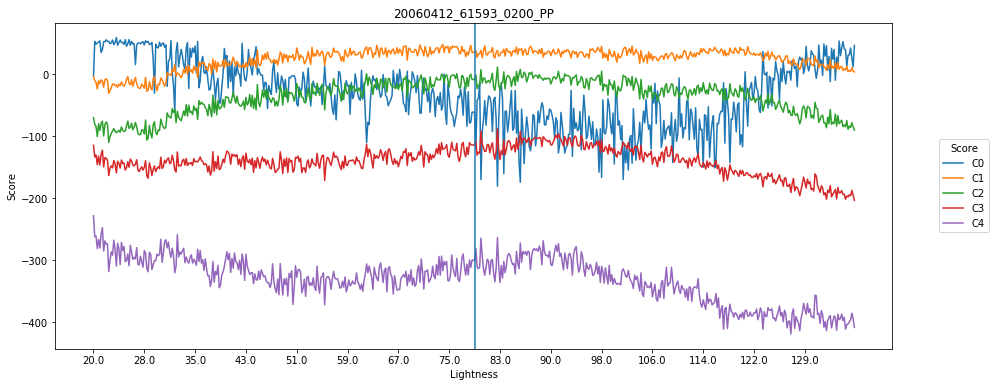
\includegraphics[width=\textwidth]{chapter_stability/20060412_61593_0200_PP/l/scores.png}
%\caption{HSL color space}
\end{figure}
\end{column}
\end{columns}
\href{run:videos_stability/Messidor_20060412_61593_0200_PP_Target_1_Checking_Hue_Sensitivity.mp4}{\color{blue}{Hue}} | \href{run:videos_stability/Messidor_20060412_61593_0200_PP_Target_1_Checking_Saturation_Sensitivity.mp4}{\color{blue}{Saturation}} | \href{run:videos_stability/Messidor_20060412_61593_0200_PP_Target_1_Checking_Luminance_Sensitivity.mp4}{\color{blue}{Lightness}}
\end{frame}

\begin{frame}{Stability analysis sample}{20060410 40481 0200 PP Target: 2 HSL}
\begin{columns}
\begin{column}{0.3\textwidth}
\begin{figure}[p]
\centering
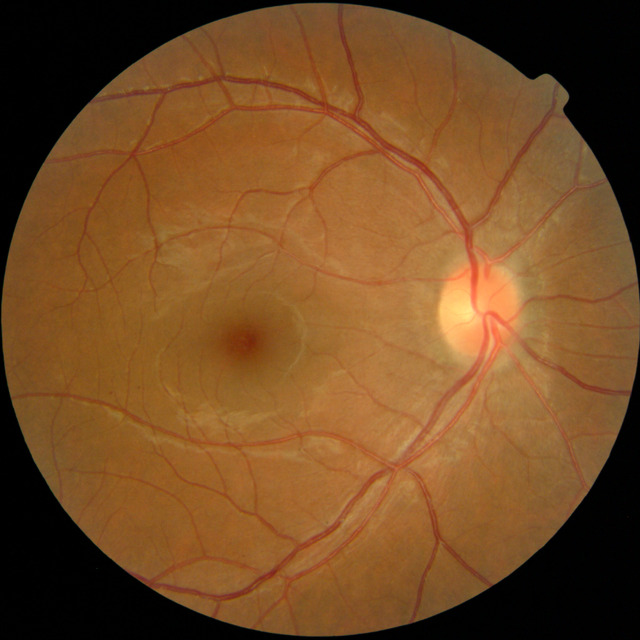
\includegraphics[width=\textwidth]{chapter_stability/20060410_40481_0200_PP/20060410_40481_0200_PP.jpeg}
%\caption{}
\end{figure}	
\end{column}
\begin{column}{0.45\textwidth}  %%<--- here
\begin{figure}[p]
\centering
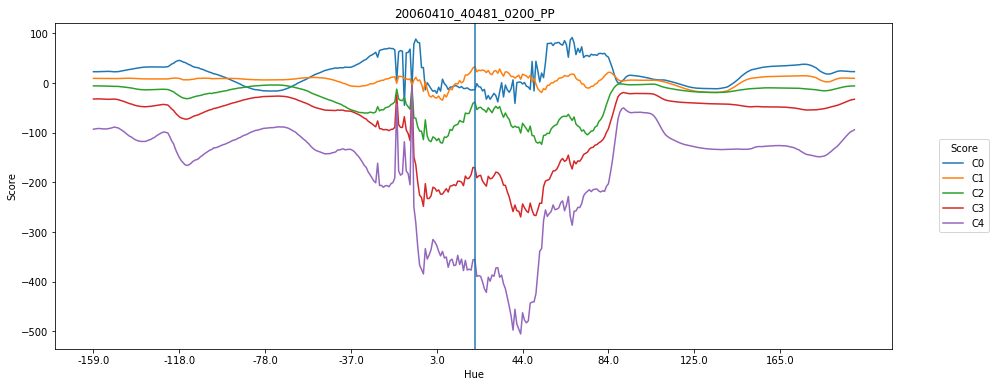
\includegraphics[width=\textwidth]{chapter_stability/20060410_40481_0200_PP/h/scores.png}			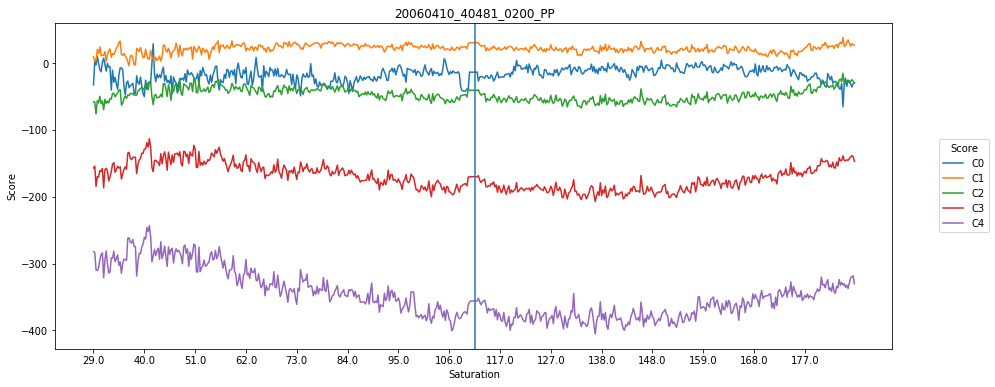
\includegraphics[width=\textwidth]{chapter_stability/20060410_40481_0200_PP/s/scores.png}			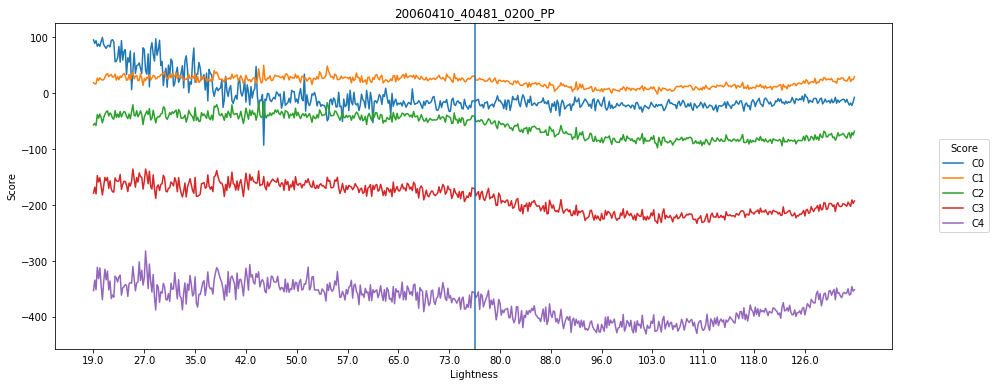
\includegraphics[width=\textwidth]{chapter_stability/20060410_40481_0200_PP/l/scores.png}
%\caption{HSL color space}
\end{figure}
\end{column}
\end{columns}
\href{run:videos_stability/Messidor_20060410_40481_0200_PP_Target_2_Checking_Hue_Sensitivity.mp4}{\color{blue}{Hue}} | \href{run:videos_stability/Messidor_20060410_40481_0200_PP_Target_2_Checking_Saturation_Sensitivity.mp4}{\color{blue}{Saturation}} | \href{run:videos_stability/Messidor_20060410_40481_0200_PP_Target_2_Checking_Luminance_Sensitivity.mp4}{\color{blue}{Lightness}}
\end{frame}


\begin{frame}{Stability analysis sample}{20051020 43906 0100 PP Target: 3 HSL}
\begin{columns}
\begin{column}{0.3\textwidth}
\begin{figure}[p]
\centering
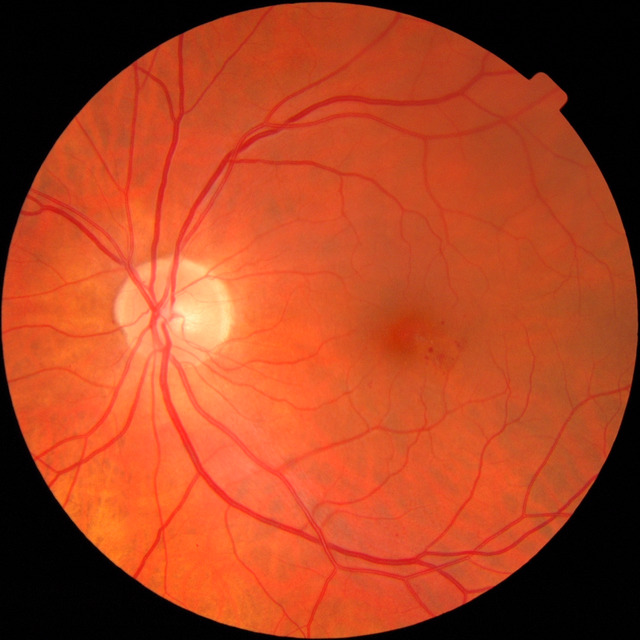
\includegraphics[width=\textwidth]{chapter_stability/20051020_43906_0100_PP/20051020_43906_0100_PP.jpeg}
%\caption{}
\end{figure}	
\end{column}
\begin{column}{0.45\textwidth}  %%<--- here
\begin{figure}[p]
\centering
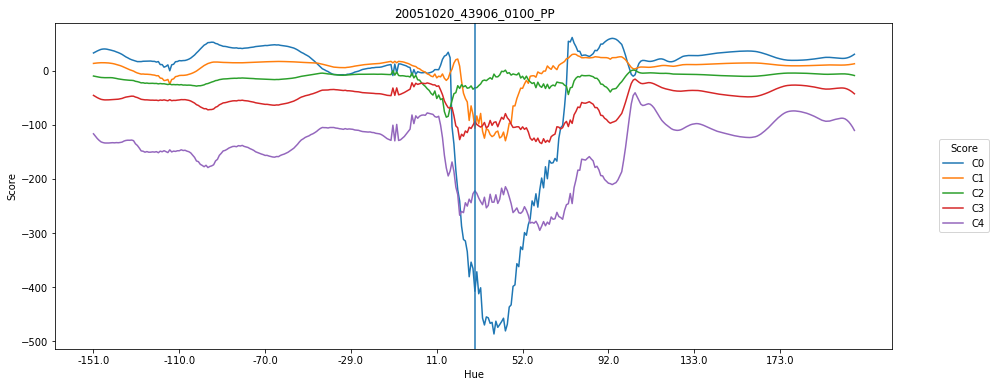
\includegraphics[width=\textwidth]{chapter_stability/20051020_43906_0100_PP/h/scores.png}			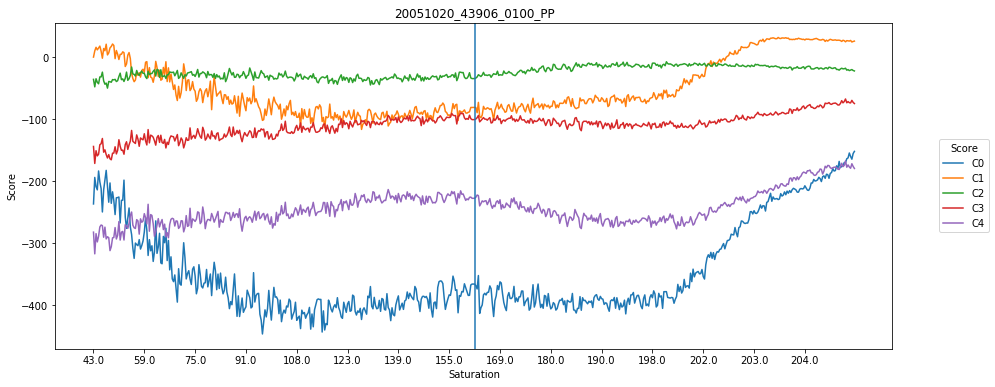
\includegraphics[width=\textwidth]{chapter_stability/20051020_43906_0100_PP/s/scores.png}			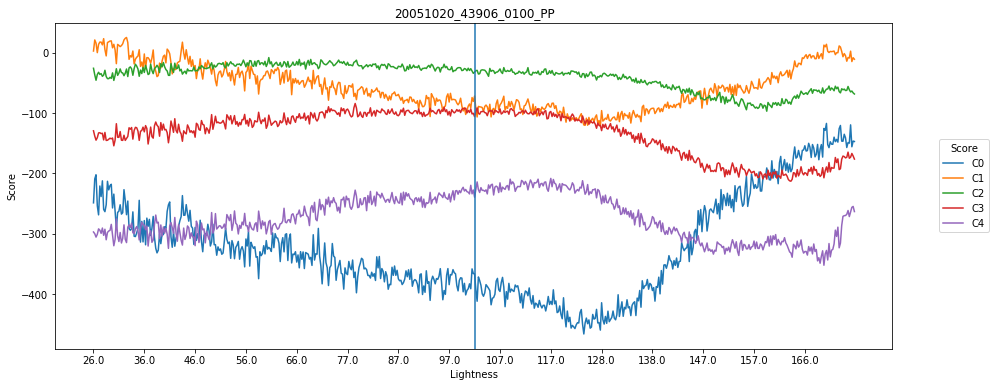
\includegraphics[width=\textwidth]{chapter_stability/20051020_43906_0100_PP/l/scores.png}
%\caption{HSL color space}
\end{figure}
\end{column}
\end{columns}
\href{run:videos_stability/Messidor_20051020_43906_0100_PP_Target_3_Checking_Hue_Sensitivity.mp4}{\color{blue}{Hue}} | \href{run:videos_stability/Messidor_20051020_43906_0100_PP_Target_3_Checking_Saturation_Sensitivity.mp4}{\color{blue}{Saturation}} | \href{run:videos_stability/Messidor_20051020_43906_0100_PP_Target_3_Checking_Luminance_Sensitivity.mp4}{\color{blue}{Lightness}}
\end{frame}


\begin{frame}{Stability analysis sample}{20060412 61593 0200 PP Target: 1 Rotation}
\begin{columns}
\begin{column}{0.3\textwidth}
\begin{figure}[p]
\centering
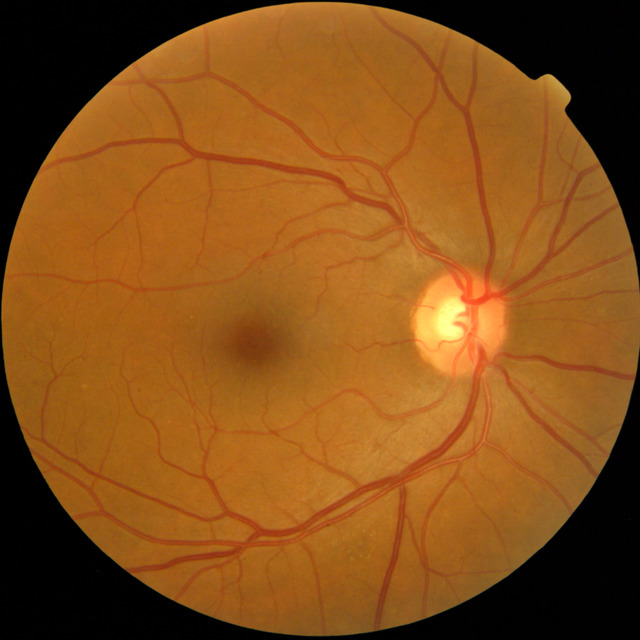
\includegraphics[width=\textwidth]{chapter_stability/20060412_61593_0200_PP/20060412_61593_0200_PP.jpeg}
%\caption{}
\end{figure}	
\end{column}
\begin{column}{0.45\textwidth}  %%<--- here
\begin{figure}[p]
\centering
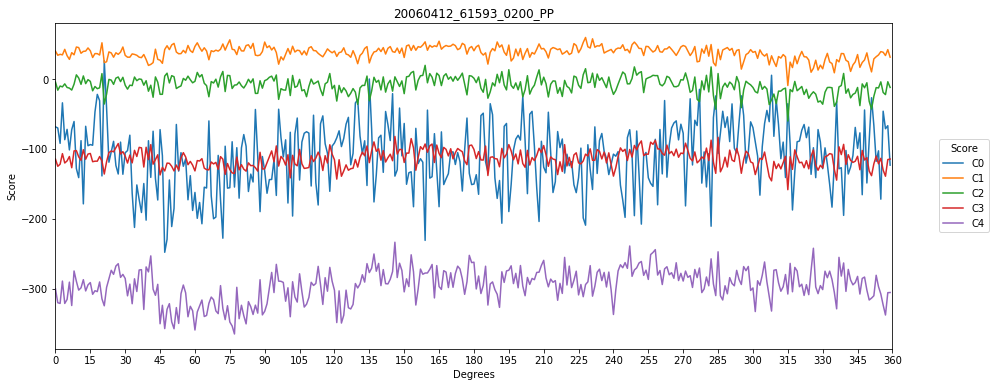
\includegraphics[width=\textwidth]{chapter_stability/20060412_61593_0200_PP/r/scores.png}
%\caption{HSL color space}
\end{figure}
\centering
\href{run:videos_stability/Messidor_20060412_61593_0200_PP_Target_1_Checking_Rotation_Sensitivity.mp4}{\color{blue}{Rotation Visualization}} 
\end{column}
\end{columns}
\end{frame}


\begin{frame}{Stability analysis sample}{20051020 44782 0100 PP Target: 1 Rotation}
\begin{columns}
\begin{column}{0.3\textwidth}
\begin{figure}[p]
\centering
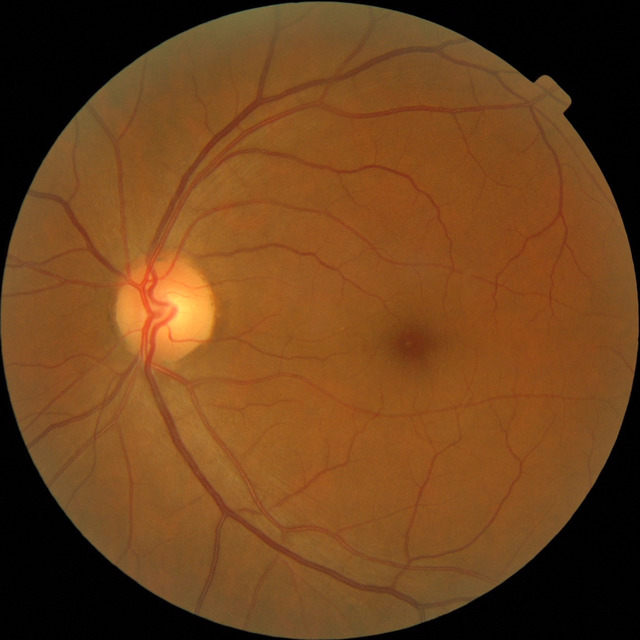
\includegraphics[width=\textwidth]{chapter_stability/20051020_44782_0100_PP/20051020_44782_0100_PP.jpeg}
%\caption{}
\end{figure}	
\end{column}
\begin{column}{0.45\textwidth}  %%<--- here
\begin{figure}[p]
\centering
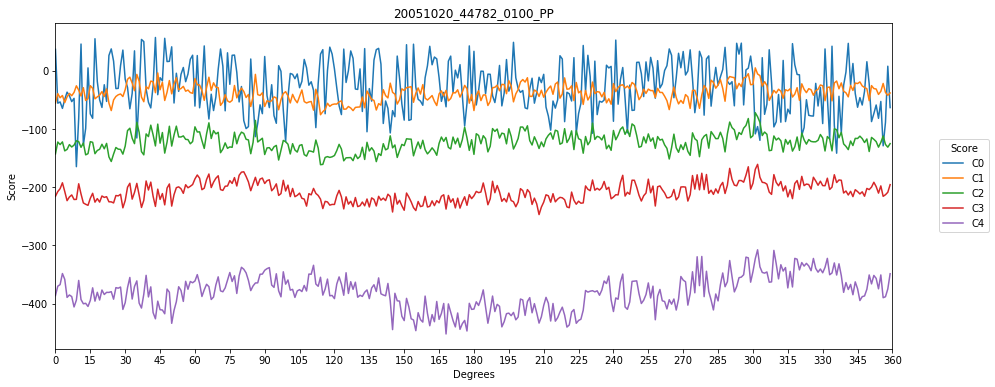
\includegraphics[width=\textwidth]{chapter_stability/20051020_44782_0100_PP/r/scores.png}
%\caption{HSL color space}
\end{figure}
\centering
\href{run:videos_stability/Messidor_20051020_44782_0100_PP_Target_1_Checking_Rotation_Sensitivity.mp4}{\color{blue}{Rotation Visualization}} 
\end{column}
\end{columns}
\end{frame}


\begin{frame}{Stability analysis sample}{20051214 57404 0100 PP Target: 2 Rotation}
\begin{columns}
\begin{column}{0.3\textwidth}
\begin{figure}[p]
\centering
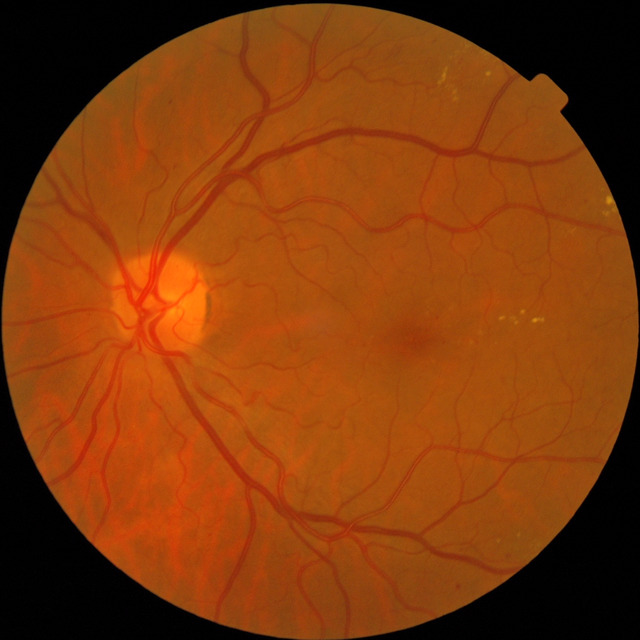
\includegraphics[width=\textwidth]{chapter_stability/20051214_57404_0100_PP/20051214_57404_0100_PP.jpeg}
%\caption{}
\end{figure}	
\end{column}
\begin{column}{0.45\textwidth}  %%<--- here
\begin{figure}[p]
\centering
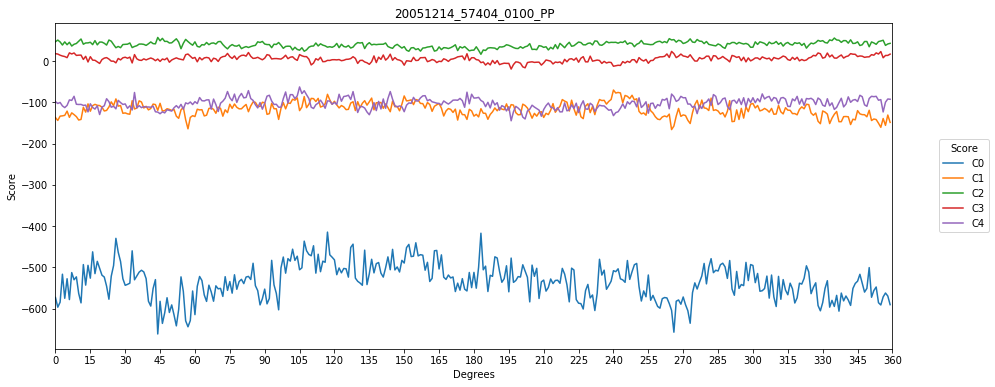
\includegraphics[width=\textwidth]{chapter_stability/20051214_57404_0100_PP/r/scores.png}
%\caption{HSL color space}
\end{figure}
\centering
\href{run:videos_stability/Messidor_20051214_57404_0100_PP_Target_2_Checking_Rotation_Sensitivity.mp4}{\color{blue}{Rotation Visualization}} 
\end{column}
\end{columns}
\end{frame}


\begin{frame}{Stability analysis sample}{20051019 38557 0100 PP Target: 3 Rotation}
\begin{columns}
\begin{column}{0.3\textwidth}
\begin{figure}[p]
\centering
\includegraphics[width=\textwidth]{chapter_stability/20051019_38557_0100_PP/20051019_38557_0100_PP.jpeg}
%\caption{}
\end{figure}	
\end{column}
\begin{column}{0.45\textwidth}  %%<--- here
\begin{figure}[p]
\centering
\includegraphics[width=\textwidth]{chapter_stability/20051019_38557_0100_PP/r/scores.png}
%\caption{HSL color space}
\end{figure}
\centering
\href{run:videos_stability/Messidor_20051019_38557_0100_PP_Target_3_Checking_Rotation_Sensitivity.mp4}{\color{blue}{Rotation Visualization}} 
\end{column}
\end{columns}
\end{frame}

\begin{frame}{Stability Conclusions}{}	
\begin{itemize}
	\item The model is stable under changes in image saturation, lightness and rotation in most of the cases.
	\item Hue camera calibration is critical for obtaining correct results.
	\item A full stability study can help improving diagnostic but requires more time.
\end{itemize}
\end{frame}

\part{Interpretation}

\section{Explanation maps generation}

\begin{frame}{Interpretation}{Objective}
Interpretation of the outputs reported by the model.
\begin{enumerate}
	\item Treat model classification outputs as scores
	\item Backpropagate them layer by layer through activated nodes until reaching input space
	\item In every layer a score map distribution of the correspondent receptive field is obtained
	\item Doing such backpropagation until reaching input space a input-space score map distribution is obtained
\end{enumerate}

\end{frame}

\begin{frame}{Interpretation}{Model}
\begin{columns}
	\begin{column}{0.5\textwidth}
\alert{Proposition 1:}
\begin{equation*}
S_l = \lambda_l a_{l}
\end{equation*}
	\end{column}
	\begin{column}{0.5\textwidth}
\alert{Proposition 2:}
\begin{equation*}
S_{l+1} = S_{l} + S_{k_l}
\end{equation*}
\end{column}
\end{columns}
\hfill \break
\alert{Score propagation scheme:}
\begin{figure}[h!]
	\centering
	\includegraphics[scale=0.85]{score_map.pdf}
%	\caption{Score distribution through layers}
\end{figure}
\alert{Score conservation equation:}
\begin{equation*}
S_L = \sum_{l=1}^L \left ( \sum S_{k_l} \right ) + \left ( \sum S_{Input} \right )
\end{equation*}
\begin{itemize}
	\item Such two propositions are enough for the derivation of a general method of score propagation.
	\item For each one of the typical deep learning blocks a score propagation model is derived.
\end{itemize}
\end{frame}

\begin{frame}{Interpretation}{Derivation of score propagation model}
\alert{Score propagation through a convolutional layer:}
\begin{columns}
	\begin{column}{0.5\textwidth}
\begin{figure}
	\centering
		\includegraphics[scale=0.55]{./chapter_interpretation/score_conv2d.pdf}
\end{figure}
	\end{column}
	\begin{column}{0.5\textwidth}
\begin{figure}
	\centering
	\includegraphics[scale=0.55]{./chapter_interpretation/score_conv2d_score.pdf}
\end{figure}		
	\end{column}
\end{columns}
\end{frame}

\begin{frame}{Interpretation}{Derivation of score propagation model}
%\alert{Score propagation through pooling layers:}
\begin{columns}
	\begin{column}{0.5\textwidth}
		\alert{Max pooling:}
		\begin{figure}
			\centering
		\includegraphics[scale=0.55]{./chapter_interpretation/score_maxpool.pdf}
		\end{figure}
	\end{column}
	\begin{column}{0.5\textwidth}
		\alert{Average pooling:}
		\begin{figure}
			\centering
		\includegraphics[scale=0.55]{./chapter_interpretation/score_avgpool.pdf}
		\end{figure}		
	\end{column}
\end{columns}
\end{frame}


\begin{frame}{Interpretation}{Derivation of score propagation model}
%\alert{Score propagation through pooling layers:}
		\alert{Fully connected layer:}
		\begin{figure}
			\centering
			\includegraphics[scale=0.95]{./chapter_interpretation/score_fc.pdf}
		\end{figure}
\end{frame}

\begin{frame}{Interpretation}{Derivation of score propagation model}
%\alert{Score propagation through pooling layers:}
\alert{Dropout layer:}
\begin{figure}
	\centering
	\includegraphics[scale=0.95]{./chapter_interpretation/score_dropout.pdf}
\end{figure}
\end{frame}

\begin{frame}{Interpretation}{Derivation of score propagation model}
\begin{columns}
	\begin{column}{0.5\textwidth}
		\alert{Score propagation through a batch normalization node:}
		\begin{figure}
			\centering
			\includegraphics{./chapter_interpretation/score_bn.pdf}
		\end{figure}		
	\end{column}

	\begin{column}{0.5\textwidth}
		\alert{Score propagation through an activation function node:}
		\begin{figure}
			\centering
			\includegraphics[width=\textwidth]{./chapter_interpretation/score_af.pdf}
		\end{figure}
	\end{column}
\end{columns}
\end{frame}

\begin{frame}{Interpretation}{Mapping the score of hidden layers and $S_k$ to input-space}
\begin{itemize}
\item Every node has two score constituents: one input-dependent, that can be easily forwarded, and another one RF-dependent, i.e layer-dependent. 

\item Effective RF is not equal to the theoretical RF \citep{luo2016understanding}. The effective one acts more like a 2D-gaussian function, where the points located in the borders contribute less than the center ones. 

\item Using such prior information, it is possible to make an approximate conversion of the full and constant scores in the hidden-space to the input-space using a 2D-gaussian prior.
\end{itemize}
\end{frame}

\begin{frame}{Interpretation}{Mapping the score of hidden layers and $S_k$ to input-space (example)}
For example, for a 20x20 hidden layer with a RF of 125x125 pixels, each point represents the cummulative value of a gaussian distribution. Summing up each gaussian distribution we obtain the map in input space.\hfill\break

\begin{columns}
	\begin{column}{0.5\textwidth}
		\alert{Hidden layer activations, RF=$125^2$:}
		\begin{figure}
			\centering
			\includegraphics[width=0.7\textwidth]{./chapter_interpretation/activations_rf125.png}
		\end{figure}		
	\end{column}
	
	\begin{column}{0.5\textwidth}
		\alert{Mapped to input-space:}
		\begin{figure}
			\centering
			\includegraphics[width=0.7\textwidth]{./chapter_interpretation/input_space_mapping_using_a_2std_gaussian_prior_rf125.png}
		\end{figure}
	\end{column}
\end{columns}

\end{frame}


%\subsection{Interpretation samples}

\begin{frame}{Interpretation}{Samples}

\begin{itemize}
	\item \href{file:///home/jordi/Escritorio/PhD-Defense-2019-presentation/interpretation_samples/model-explanations-score-propagation-rev4_sample2_class4.html}{\color{blue}{Class 4 score feature-wise visualization propagation}}
	\item \href{file:///home/jordi/Escritorio/PhD-Defense-2019-presentation/interpretation_samples/model-explanations-score-propagation-rev5_sample1_class4.html}{\color{blue}{Class 4 score layer-wise visualization propagation}}
\end{itemize}
\begin{columns}
	\begin{column}{0.5\textwidth}
\begin{itemize}
\item \href{file:///home/jordi/Escritorio/PhD-Defense-2019-presentation/videos_scores/11736_left.mp4}{Class 1: 11736 left}
\item \href{file:///home/jordi/Escritorio/PhD-Defense-2019-presentation/videos_scores/11854_left.mp4}{Class 4: 11854 left}
\item \href{file:///home/jordi/Escritorio/PhD-Defense-2019-presentation/videos_scores/1561_left.mp4}{Class 3: 1561 left}
\item \href{file:///home/jordi/Escritorio/PhD-Defense-2019-presentation/videos_scores/162_right.mp4}{Class 0: 162 right}
\item \href{file:///home/jordi/Escritorio/PhD-Defense-2019-presentation/videos_scores/20051019_38557_0100_PP.mp4}{Class 2: 20051019 38557}
\item \href{file:///home/jordi/Escritorio/PhD-Defense-2019-presentation/videos_scores/20051020_43906_0100_PP.mp4}{Class 2: 20051020 43906}
\item \href{file:///home/jordi/Escritorio/PhD-Defense-2019-presentation/videos_scores/20051021_52127_0100_PP.mp4}{Class 2: 20051021 52127}
\item \href{file:///home/jordi/Escritorio/PhD-Defense-2019-presentation/videos_scores/20051214_57404_0100_PP.mp4}{Class 2: 20051214 57404}
\end{itemize}
\end{column}
	\begin{column}{0.5\textwidth}
\begin{itemize}
\item \href{file:///home/jordi/Escritorio/PhD-Defense-2019-presentation/videos_scores/20051216_44939_0200_PP.mp4}{Class 2: 20051216 44939}
\item \href{file:///home/jordi/Escritorio/PhD-Defense-2019-presentation/videos_scores/20060410_40481_0200_PP.mp4}{Class 1: 20060410 40481}
\item \href{file:///home/jordi/Escritorio/PhD-Defense-2019-presentation/videos_scores/20060411_62228_0200_PP.mp4}{Class 1: 20060411 62228}
\item \href{file:///home/jordi/Escritorio/PhD-Defense-2019-presentation/videos_scores/20060412_59658_0200_PP.mp4}{Class 1: 20060412 59658}
\item \href{file:///home/jordi/Escritorio/PhD-Defense-2019-presentation/videos_scores/20060412_59717_0200_PP.mp4}{Class 2: 20060412 59717}
\item \href{file:///home/jordi/Escritorio/PhD-Defense-2019-presentation/videos_scores/20060412_61593_0200_PP.mp4}{Class 1: 20060412 61593}
\item \href{file:///home/jordi/Escritorio/PhD-Defense-2019-presentation/videos_scores/20060523_45524_0100_PP.mp4}{Class 0: 20060523 45524}
\item \href{file:///home/jordi/Escritorio/PhD-Defense-2019-presentation/videos_scores/20060523_50392_0100_PP.mp4}{Class 2: 20060523 50392}
\end{itemize}
	\end{column}
\end{columns}
\end{frame}

\begin{frame}{Interpretation}{Conclusions}	
\begin{itemize}
	\item We designed a method for deep learning models result interpretation based on input-space score map generation
	\item The model is designed for general applicability in different domains and for different networks
	\item We show an application based on interpretation of the results reported in our diabetic retinopathy disease grading model.
	\item The interpretation model is able to identify correctly the lesions present in images.
	\item Such identification is inferred only from the information coming from the disease grading labels of the training set
	\item This results prove, not only that the interpretation model is successful in determining the causes under a particular classification but also that the original model is able to identify the important features of the image, ie. the correct statistical regularities.
\end{itemize}
\end{frame}

\section{Feature Space Compression}

\begin{frame}{Feature Space Compression}{}
\begin{itemize}
\item Neural networks feature spaces are frequently high-dimensional with high correlation values between  dimensions, ie. are low dimensional manifolds embedded in high dimensional spaces.
\item We present a methodology for linear compression of the feature space allowing the feature space compression from the original 64 dimensions to only 3 with a reduction of performance lower than 2.5\%.
\item This feature-space compression aims to facilitate the interpretation.
\end{itemize}
\end{frame}

\begin{frame}{Feature Space Compression}{Methodology}
\alert{Initial Classifier}
\begin{figure}
	\centering
	\includegraphics[width=0.75\textwidth]{chapter_ica/initial_classifier.pdf}
\end{figure}
\alert{Modified Classifier}
\begin{figure}
	\centering
	\includegraphics[width=\textwidth]{chapter_ica/ica_classifier.pdf}
\end{figure}

\end{frame}


\begin{frame}{Feature Space Compression}{Mathematical Formalization}

		\begin{equation}
		F_{train} = \{\boldsymbol{f^{(i)}} : i = 1 .. T\}, \quad \boldsymbol{f^{(i)}} = (f^{(i)}_1, f^{(i)}_2, ... f^{(i)}_m)
		\end{equation}
		
		\begin{equation}
		S_{train} = \{\boldsymbol{s^{(i)}} : i = 1 .. T\}, \quad \boldsymbol{s^{(i)}} = (s^{(i)}_1, s^{(i)}_2, ... s^{(i)}_n)
		\end{equation}
		
		\begin{equation}
		\boldsymbol{s^{(i)}} = \boldsymbol{W} \boldsymbol{f^{(i)}}
		\end{equation}
		
		\begin{equation}
		\max_{\boldsymbol{A}} \big[ \kappa_{val} (C_{train}) \big]
		\end{equation}
		
		\begin{equation}
		C_{train} = \{ \boldsymbol{A} \boldsymbol{f^{(i)}}, \forall \boldsymbol{f^{(i)}} \in F_{train} \} 
		\end{equation}

		\begin{equation}
		C'_{train} = \{ \boldsymbol{B} \boldsymbol{s^{(i)}}, \forall \boldsymbol{s^{(i)}} \in S_{train} \} 
		\end{equation}
		
		\begin{equation}
		\min_{n} \big[ \kappa_{val} (C'_{train}) - \kappa_{val} (C_{train}) \big] 
		\end{equation}
\end{frame}


\begin{frame}{Feature Space Compression}{}
\alert{Comparison between the 2D t-SNE visualization of validation set using the original feature space and the final 3-dimensional ICA space:}
\begin{figure}[h]
	\centering
	\begin{subfigure}[b]{0.49\textwidth}
		\centering
		\includegraphics[width=\textwidth]{./chapter_ica/tsne2d_p75.eps}
		\caption{Original feature space (64 comp.)}	
	\end{subfigure}
	\begin{subfigure}[b]{0.49\textwidth}
		\centering
		\includegraphics[width=\textwidth]{./chapter_ica/tsne2d_ica_p75.eps}
		\caption{ICA space (3 comp.)}
	\end{subfigure}	
	%\caption{}  
	\label{fig:tsne} 
\end{figure}
\end{frame}

%\begin{frame}{Feature Space Compression}{ICA Class Contribution}
%\begin{figure}[h]
%	\centering
%	\includegraphics[width=\textwidth]{chapter_ica/ica_class_contribution.eps}
%\end{figure}
%\end{frame}

\begin{frame}{Feature space compression}{Conclusions}	
\begin{itemize}
	\item We designed a method for the internal compression of the feature space model representation
	\item The method is of general applicability to other networks and applications
	\item In the diabetic retinopathy disease grading case the method allows the compression of the original 64 features internal representation into only 3 features with a loss of perfomance lower than 2.5\%.
	\item Reducing the number of features and the correlation between them, facilitates its interpretation by human experts.
 \end{itemize}
\end{frame}

\part{Application and Conclusions}

\section{Experimental Application}

\begin{frame}{Experimental Application}{Inference using HUSJR data}
\begin{itemize}
	\item The objective of this study is determine the applicability of the designed model for the prediction in a real case of the Hospital Universitari Sant Joan de Reus.
	\item For this purpose a database of $19,230$ tagged retinographies is used.
	\item Some discrepancies are detected in the definition of the classes used in HUSJR and the ones of the trained model.
	\item After an initial evaluation with original model a retraining is applied for making compatible the class definitions.
	\item Messidor-2 class definition is defined as the new standard.
	\item Last linear classification layer is retrained.
\end{itemize}
\end{frame}

\begin{frame}{Experimental Application}{Inference using HUSJR data}
\alert{t-SNE visualization of the feature space representation of samples of HUSJR dataset. Blue (class 0), green (class 1), yellow (class 2) and red (class 3)}
\begin{figure}
	\centering
	\includegraphics[width=0.5\textwidth]{chapter_reus/feature_space_reus.png}
\end{figure}
\end{frame}

\begin{frame}{Experimental Application}{Inference using HUSJR data}
\alert{HUSJR confusion matrix using EyePACS trained original model. $QWK = 0.791$ }
\begin{table}[ht]
	\centering
	\scalebox{0.85}{
		\begin{tabular}{c|ccccc}
			\hline
			& Pred 0 & Pred 1 & Pred 2 & Pred 3 & Pred 4\\ \hline
			True 0 &  15,112 &   2,024 &     159 &      6  &      12\\ 
			True 1 &      11 &     547 &     326 &     14  &       3\\ 
			True 2 &       0 &       4 &     439 &    133  &       7\\ 
			True 3 &       0 &       1 &      20 &    358  &      54\\ 
			\hline	
		\end{tabular}
	}
\end{table}

\alert{HUSJR confusion matrix with EyePACS trained original model plus a linear classifier retrained using Messidor-2 Dataset. $QWK = 0.823$}

\begin{table}[ht]
	\centering
	\scalebox{1.0}{
		\begin{tabular}{c|ccccc}
			\hline
			& Pred 0 & Pred 1 & Pred 2 & Pred 3\\ \hline
			True 0 &  15,277 &   1,944 &      83 &      9 \\ 
			True 1 &       5 &     595 &     284 &     17 \\ 
			True 2 &       0 &       2 &     456 &    125 \\ 
			True 3 &       0 &       1 &       6 &    426 \\ 
			\hline	
		\end{tabular}
	}
\end{table}

\end{frame}

\begin{frame}{Experimental Application}{Inference using HUSJR data}
The indexes obtained for classification of the most severe cases of the disease (considering positive class = 2,3 and negative class = 0,1) are:
\begin{itemize}
	\item Sensitivity = 0.997
	\item Specificity = 0.978
	\item Positive predictive value (PPV) = 0.720
	\item Negative predictive value (NPV) = 0.9998
	\item Accuracy (ACC) = 0.979
	\item $F_1$ Score = 0.836
\end{itemize}
\end{frame}

\begin{frame}{Experimental Application}{Conclusions of inference using HUSJR data}
\begin{itemize}
	\item We studied the applicability of our best model for the prediction of diabetic retinopathy, trained using the EyePACS dataset, for the prediction of diabetic retinopathy in HUSJR
	\item A feature space visualization has been done in order to check its capacity for separating between classes.
	\item A first evaluation of the model predictability was done, obtaining good results, but with small loss in performance. This loss was probably produced to the slight differences in class definitions.
	\item After a class standardization, the linear classifier of the model was retrained using Messidor-2 Dataset, using as a feature extractor the original model.
	\item  Performance of the new model was tested again, reaching values of inter-rater agreement similar to the obtained by expert ophthalmologists.
	\item Medical team is extremely satisfied with obtained results.
\end{itemize}
\end{frame}

\section{Contributions}

\begin{frame}{Summary of contributions I}{The main contributions of this thesis are:}

\begin{enumerate}
	\item Design of automatic classifiers based on deep neural networks able to reach ophthalmologist performance level.
	
	\fullcite{jdelatorre2016}
	
\end{enumerate}
\end{frame}

\begin{frame}{Summary of contributions II}{The main contributions of this thesis are:}

\begin{enumerate}
	\setcounter{enumi}{1}
		
	\item Study of the usage of Quadratic Weighted Kappa index as a Deep Learning Loss Function for the optimization of ordinal regression problems.

	\fullcite{delatorre2017} Impact Factor: 1.952 (Q2)

	\item Study of the feature space manifold stability of the designed diabetic retinopathy classifiers.
	
	\item Design of a generalized model for the interpretation of results reported by deep learning classifiers.
	
	\fullcite{de2017deep} Accepted for publication in \emph{Neurocomputing}. Impact Factor: 3.241 (Q1)	
\end{enumerate}
\end{frame}


\begin{frame}{Summary of contributions III}{The main contributions of this thesis are:}

\begin{enumerate}
	\setcounter{enumi}{4}
	
	\item Design of a method for compressing feature space internal representations of deep learning models.
	
	\fullcite{delatorre_ica_2018} \\Under revision in \emph{Computer Methods and Programs in Biomedicine}. Impact Factor: 2.674 (Q2)
	
	\item Application of designed classifiers into a real use case in Hospital de Reus. A software has been implemented for DR classification and lesion identification. Registered in Benelux Office for Intellectual Property. Reference number 109999.	
\end{enumerate}
\end{frame}

%\begin{frame}{Summary of contributions}{}	
%\begin{itemize}
%	\item We designed a diabetic retinopathy automatic classifier based on convolutional neural networks able to diagnose the disease grading with the information reported by a retinography achieving inter-rater agreements close to the reported by trained professionals.
%	\item We studied the stability of the proposed model for changes in rotation and color space, experimentally proving the robustness of the prediction algorithm.
%	\item We proposed a new loss function for the optimization of ordinal regression problems that is able to achieve increases of performance in deep learning based models between 5-10\% over the standard log-loss.
%	\item We proposed a new interpretation method for the result explanations given by deep learning models. This method have been tested using the diabetic retinopathy classifiers designed in this thesis with excellent results. Being a method of general applicability it is expected to be used also in other domains.
%	\item We tested the applicability of designed models for the prediction in real cases, obtaining promising results.
%\end{itemize}	
%\end{frame}

\section{Future research lines}

\begin{frame}{Future possible research lines}{}	
\begin{itemize}
	\item Increase the number of classes to predict
	\item Transfer learning: Successful networks in challenging tasks like ImageNet, can be good candidates to perform well in specialized medical imaging tasks like ours.
	\item Unsupervised learning: Generative Adversarial Networks can also be
	explored for generating new high quality samples from the original dataset
	\item Reinforcement Learning: Adding to the models the possibility of enhancing its performance, designing online learning methods that allow continuous learning of networks from the corrections done by ophthalmologists on inference time
	\item Use of Interpretation Model in other applications
	\item Interpretation model for unsupervised image segmentation
\end{itemize}	
\end{frame}


\begin{frame}{}
\centering
\huge Thank you.
\end{frame}

\begin{frame}{Stability analysis sample}{20060523 45524 0100 PP Target: 0 HSL}
\begin{columns}
	\begin{column}{0.3\textwidth}
		\begin{figure}[p]
			\centering
			\includegraphics[width=\textwidth]{chapter_stability/20060523_45524_0100_PP/20060523_45524_0100_PP.jpeg}
			%\caption{}
		\end{figure}	
	\end{column}
	\begin{column}{0.45\textwidth}  %%<--- here
		\begin{figure}[p]
			\centering
			\includegraphics[width=\textwidth]{chapter_stability/20060523_45524_0100_PP/h/scores.png}			\includegraphics[width=\textwidth]{chapter_stability/20060523_45524_0100_PP/s/scores.png}			\includegraphics[width=\textwidth]{chapter_stability/20060523_45524_0100_PP/l/scores.png}
			%\caption{HSL color space}
		\end{figure}
	\end{column}
\end{columns}
\href{run:videos_stability/Messidor_20060523_45524_0100_PP_Target_0_Checking_Hue_Sensitivity.mp4}{\color{blue}{Hue}} | \href{run:videos_stability/Messidor_20060523_45524_0100_PP_Target_0_Checking_Saturation_Sensitivity.mp4}{\color{blue}{Saturation}} | \href{run:videos_stability/Messidor_20060523_45524_0100_PP_Target_0_Checking_Luminance_Sensitivity.mp4}{\color{blue}{Lightness}}
\end{frame}

\begin{frame}{Stability analysis sample}{20060411 62228 0200 PP Target: 1 HSL}
\begin{columns}
	\begin{column}{0.3\textwidth}
		\begin{figure}[p]
			\centering
			\includegraphics[width=\textwidth]{chapter_stability/20060411_62228_0200_PP/20060411_62228_0200_PP.jpeg}
			%\caption{}
		\end{figure}	
	\end{column}
	\begin{column}{0.45\textwidth}  %%<--- here
		\begin{figure}[p]
			\centering
			\includegraphics[width=\textwidth]{chapter_stability/20060411_62228_0200_PP/h/scores.png}			\includegraphics[width=\textwidth]{chapter_stability/20060411_62228_0200_PP/s/scores.png}			\includegraphics[width=\textwidth]{chapter_stability/20060411_62228_0200_PP/l/scores.png}
			%\caption{HSL color space}
		\end{figure}
	\end{column}
\end{columns}
\href{run:videos_stability/Messidor_20060411_62228_0200_PP_Target_1_Checking_Hue_Sensitivity.mp4}{\color{blue}{Hue}} | \href{run:videos_stability/Messidor_20060411_62228_0200_PP_Target_1_Checking_Saturation_Sensitivity.mp4}{\color{blue}{Saturation}} | \href{run:videos_stability/Messidor_20060411_62228_0200_PP_Target_1_Checking_Luminance_Sensitivity.mp4}{\color{blue}{Lightness}}
\end{frame}

\begin{frame}{Stability analysis sample}{20051020 44782 0100 PP Target: 1 HSL}
\begin{columns}
	\begin{column}{0.3\textwidth}
		\begin{figure}[p]
			\centering
			\includegraphics[width=\textwidth]{chapter_stability/20051020_44782_0100_PP/20051020_44782_0100_PP.jpeg}
			%\caption{}
		\end{figure}	
	\end{column}
	\begin{column}{0.45\textwidth}  %%<--- here
		\begin{figure}[p]
			\centering
			\includegraphics[width=\textwidth]{chapter_stability/20051020_44782_0100_PP/h/scores.png}			\includegraphics[width=\textwidth]{chapter_stability/20051020_44782_0100_PP/s/scores.png}			\includegraphics[width=\textwidth]{chapter_stability/20051020_44782_0100_PP/l/scores.png}
			%\caption{HSL color space}
		\end{figure}
	\end{column}
\end{columns}
\href{run:videos_stability/Messidor_20051020_44782_0100_PP_Target_1_Checking_Hue_Sensitivity.mp4}{\color{blue}{Hue}} | \href{run:videos_stability/Messidor_20051020_44782_0100_PP_Target_1_Checking_Saturation_Sensitivity.mp4}{\color{blue}{Saturation}} | \href{run:videos_stability/Messidor_20051020_44782_0100_PP_Target_1_Checking_Luminance_Sensitivity.mp4}{\color{blue}{Lightness}}
\end{frame}

\begin{frame}{Stability analysis sample}{20051214 57404 0100 PP Target: 2 HSL}
\begin{columns}
	\begin{column}{0.3\textwidth}
		\begin{figure}[p]
			\centering
			\includegraphics[width=\textwidth]{chapter_stability/20051214_57404_0100_PP/20051214_57404_0100_PP.jpeg}
			%\caption{}
		\end{figure}	
	\end{column}
	\begin{column}{0.45\textwidth}  %%<--- here
		\begin{figure}[p]
			\centering
			\includegraphics[width=\textwidth]{chapter_stability/20051214_57404_0100_PP/h/scores.png}			\includegraphics[width=\textwidth]{chapter_stability/20051214_57404_0100_PP/s/scores.png}			\includegraphics[width=\textwidth]{chapter_stability/20051214_57404_0100_PP/l/scores.png}
			%\caption{HSL color space}
		\end{figure}
	\end{column}
\end{columns}
\href{run:videos_stability/Messidor_20051214_57404_0100_PP_Target_2_Checking_Hue_Sensitivity.mp4}{\color{blue}{Hue}} | \href{run:videos_stability/Messidor_20051214_57404_0100_PP_Target_2_Checking_Saturation_Sensitivity.mp4}{\color{blue}{Saturation}} | \href{run:videos_stability/Messidor_20051214_57404_0100_PP_Target_2_Checking_Luminance_Sensitivity.mp4}{\color{blue}{Lightness}}
\end{frame}

\begin{frame}{Stability analysis sample}{20051216 44939 0200 PP Target: 2 HSL}
\begin{columns}
\begin{column}{0.3\textwidth}
	\begin{figure}[p]
		\centering
		\includegraphics[width=\textwidth]{chapter_stability/20051216_44939_0200_PP/20051216_44939_0200_PP.jpeg}
		%\caption{}
	\end{figure}	
\end{column}
\begin{column}{0.45\textwidth}  %%<--- here
	\begin{figure}[p]
		\centering
		\includegraphics[width=\textwidth]{chapter_stability/20051216_44939_0200_PP/h/scores.png}			\includegraphics[width=\textwidth]{chapter_stability/20051216_44939_0200_PP/s/scores.png}			\includegraphics[width=\textwidth]{chapter_stability/20051216_44939_0200_PP/l/scores.png}
		%\caption{HSL color space}
	\end{figure}
\end{column}
\end{columns}
\href{run:videos_stability/Messidor_20051216_44939_0200_PP_Target_2_Checking_Hue_Sensitivity.mp4}{\color{blue}{Hue}} | \href{run:videos_stability/Messidor_20051216_44939_0200_PP_Target_2_Checking_Saturation_Sensitivity.mp4}{\color{blue}{Saturation}} | \href{run:videos_stability/Messidor_20051216_44939_0200_PP_Target_2_Checking_Luminance_Sensitivity.mp4}{\color{blue}{Lightness}}
\end{frame}

\begin{frame}{Stability analysis sample}{20060412 59717 0200 PP Target: 3 HSL}
\begin{columns}
	\begin{column}{0.3\textwidth}
		\begin{figure}[p]
			\centering
			\includegraphics[width=\textwidth]{chapter_stability/20060412_59717_0200_PP/20060412_59717_0200_PP.jpeg}
			%\caption{}
		\end{figure}	
	\end{column}
	\begin{column}{0.45\textwidth}  %%<--- here
		\begin{figure}[p]
			\centering
			\includegraphics[width=\textwidth]{chapter_stability/20060412_59717_0200_PP/h/scores.png}			\includegraphics[width=\textwidth]{chapter_stability/20060412_59717_0200_PP/s/scores.png}			\includegraphics[width=\textwidth]{chapter_stability/20060412_59717_0200_PP/l/scores.png}
			%\caption{HSL color space}
		\end{figure}
	\end{column}
\end{columns}
\href{run:videos_stability/Messidor_20060412_59717_0200_PP_Target_3_Checking_Hue_Sensitivity.mp4}{\color{blue}{Hue}} | \href{run:videos_stability/Messidor_20060412_59717_0200_PP_Target_3_Checking_Saturation_Sensitivity.mp4}{\color{blue}{Saturation}} | \href{run:videos_stability/Messidor_20060412_59717_0200_PP_Target_3_Checking_Luminance_Sensitivity.mp4}{\color{blue}{Lightness}}
\end{frame}

\begin{frame}{Stability analysis sample}{20051019 38557 0100 PP Target: 3 HSL}
\begin{columns}
\begin{column}{0.3\textwidth}
	\begin{figure}[p]
		\centering
		\includegraphics[width=\textwidth]{chapter_stability/20051019_38557_0100_PP/20051019_38557_0100_PP.jpeg}
		%\caption{}
	\end{figure}	
\end{column}
\begin{column}{0.45\textwidth}  %%<--- here
	\begin{figure}[p]
		\centering
		\includegraphics[width=\textwidth]{chapter_stability/20051019_38557_0100_PP/h/scores.png}			\includegraphics[width=\textwidth]{chapter_stability/20051019_38557_0100_PP/s/scores.png}			\includegraphics[width=\textwidth]{chapter_stability/20051019_38557_0100_PP/l/scores.png}
		%\caption{HSL color space}
	\end{figure}
\end{column}
\end{columns}
\href{run:videos_stability/Messidor_20051019_38557_0100_PP_Target_3_Checking_Hue_Sensitivity.mp4}{\color{blue}{Hue}} | \href{run:videos_stability/Messidor_20051019_38557_0100_PP_Target_3_Checking_Saturation_Sensitivity.mp4}{\color{blue}{Saturation}} | \href{run:videos_stability/Messidor_20051019_38557_0100_PP_Target_3_Checking_Luminance_Sensitivity.mp4}{\color{blue}{Lightness}}
\end{frame}

\begin{frame}{Stability analysis sample}{20051019 38557 0100 PP Target: 3 Rotation}
\begin{columns}
	\begin{column}{0.3\textwidth}
		\begin{figure}[p]
			\centering
			\includegraphics[width=\textwidth]{chapter_stability/20051019_38557_0100_PP/20051019_38557_0100_PP.jpeg}
			%\caption{}
		\end{figure}	
	\end{column}
	\begin{column}{0.45\textwidth}  %%<--- here
		\begin{figure}[p]
			\centering
			\includegraphics[width=\textwidth]{chapter_stability/20051019_38557_0100_PP/r/scores.png}
			%\caption{HSL color space}
		\end{figure}
		\centering
		\href{run:videos_stability/Messidor_20051019_38557_0100_PP_Target_3_Checking_Rotation_Sensitivity.mp4}{\color{blue}{Rotation Visualization}} 
	\end{column}
\end{columns}
\end{frame}

\begin{frame}{Stability analysis sample}{20060411 62228 0200 PP Target: 1 Rotation}
\begin{columns}
	\begin{column}{0.3\textwidth}
		\begin{figure}[p]
			\centering
			\includegraphics[width=\textwidth]{chapter_stability/20060411_62228_0200_PP/20060411_62228_0200_PP.jpeg}
			%\caption{}
		\end{figure}	
	\end{column}
	\begin{column}{0.45\textwidth}  %%<--- here
		\begin{figure}[p]
			\centering
			\includegraphics[width=\textwidth]{chapter_stability/20060411_62228_0200_PP/r/scores.png}
			%\caption{HSL color space}
		\end{figure}
		\centering
		\href{run:videos_stability/Messidor_20060411_62228_0200_PP_Target_1_Checking_Rotation_Sensitivity.mp4}{\color{blue}{Rotation Visualization}} 
	\end{column}
\end{columns}
\end{frame}

\begin{frame}{Stability analysis sample}{20060412 59658 0200 PP Target: 1 Rotation}
\begin{columns}
	\begin{column}{0.3\textwidth}
		\begin{figure}[p]
			\centering
			\includegraphics[width=\textwidth]{chapter_stability/20060412_59658_0200_PP/20060412_59658_0200_PP.jpeg}
			%\caption{}
		\end{figure}	
	\end{column}
	\begin{column}{0.45\textwidth}  %%<--- here
		\begin{figure}[p]
			\centering
			\includegraphics[width=\textwidth]{chapter_stability/20060412_59658_0200_PP/r/scores.png}
			%\caption{HSL color space}
		\end{figure}
		\centering
		\href{run:videos_stability/Messidor_20060412_59658_0200_PP_Target_1_Checking_Rotation_Sensitivity.mp4}{\color{blue}{Rotation Visualization}} 
	\end{column}
\end{columns}
\end{frame}

\begin{frame}{Stability analysis sample}{20060410 40481 0200 PP Target: 1 Rotation}
\begin{columns}
	\begin{column}{0.3\textwidth}
		\begin{figure}[p]
			\centering
			\includegraphics[width=\textwidth]{chapter_stability/20060410_40481_0200_PP/20060410_40481_0200_PP.jpeg}
			%\caption{}
		\end{figure}	
	\end{column}
	\begin{column}{0.45\textwidth}  %%<--- here
		\begin{figure}[p]
			\centering
			\includegraphics[width=\textwidth]{chapter_stability/20060410_40481_0200_PP/r/scores.png}
			%\caption{HSL color space}
		\end{figure}
		\centering
		\href{run:videos_stability/Messidor_20060410_40481_0200_PP_Target_1_Checking_Rotation_Sensitivity.mp4}{\color{blue}{Rotation Visualization}} 
	\end{column}
\end{columns}
\end{frame}

\begin{frame}{Stability analysis sample}{20060523 50392 0100 PP Target: 2 Rotation}
\begin{columns}
\begin{column}{0.3\textwidth}
	\begin{figure}[p]
		\centering
		\includegraphics[width=\textwidth]{chapter_stability/20060523_50392_0100_PP/20060523_50392_0100_PP.jpeg}
		%\caption{}
	\end{figure}	
\end{column}
\begin{column}{0.45\textwidth}  %%<--- here
	\begin{figure}[p]
		\centering
		\includegraphics[width=\textwidth]{chapter_stability/20060523_50392_0100_PP/r/scores.png}
		%\caption{HSL color space}
	\end{figure}
	\centering
	\href{run:videos_stability/Messidor_20060523_50392_0100_PP_Target_2_Checking_Rotation_Sensitivity.mp4}{\color{blue}{Rotation Visualization}} 
\end{column}
\end{columns}
\end{frame}


\begin{frame}{Stability analysis sample}{20051020 43906 0100 PP Target: 3 Rotation}
\begin{columns}
	\begin{column}{0.3\textwidth}
		\begin{figure}[p]
			\centering
			\includegraphics[width=\textwidth]{chapter_stability/20051020_43906_0100_PP/20051020_43906_0100_PP.jpeg}
			%\caption{}
		\end{figure}	
	\end{column}
	\begin{column}{0.45\textwidth}  %%<--- here
		\begin{figure}[p]
			\centering
			\includegraphics[width=\textwidth]{chapter_stability/20051020_43906_0100_PP/r/scores.png}
			%\caption{HSL color space}
		\end{figure}
		\centering
		\href{run:videos_stability/Messidor_20051020_43906_0100_PP_Target_3_Checking_Rotation_Sensitivity.mp4}{\color{blue}{Rotation Visualization}} 
	\end{column}
\end{columns}
\end{frame}

\begin{frame}{Stability analysis sample}{20051021 52127 0100 PP Target: 3 Rotation}
\begin{columns}
\begin{column}{0.3\textwidth}
	\begin{figure}[p]
		\centering
		\includegraphics[width=\textwidth]{chapter_stability/20051021_52127_0100_PP/20051021_52127_0100_PP.jpeg}
		%\caption{}
	\end{figure}	
\end{column}
\begin{column}{0.45\textwidth}  %%<--- here
	\begin{figure}[p]
		\centering
		\includegraphics[width=\textwidth]{chapter_stability/20051021_52127_0100_PP/r/scores.png}
		%\caption{HSL color space}
	\end{figure}
	\centering
	\href{run:videos_stability/Messidor_20051021_52127_0100_PP_Target_3_Checking_Rotation_Sensitivity.mp4}{\color{blue}{Rotation Visualization}} 
\end{column}
\end{columns}
\end{frame}

\begin{frame}{Stability analysis sample}{20060412 59717 0200 PP Target: 3 Rotation}
\begin{columns}
\begin{column}{0.3\textwidth}
\begin{figure}[p]
	\centering
	\includegraphics[width=\textwidth]{chapter_stability/20060412_59717_0200_PP/20060412_59717_0200_PP.jpeg}
	%\caption{}
\end{figure}	
\end{column}
\begin{column}{0.45\textwidth}  %%<--- here
\begin{figure}[p]
	\centering
	\includegraphics[width=\textwidth]{chapter_stability/20060412_59717_0200_PP/r/scores.png}
	%\caption{HSL color space}
\end{figure}
\centering
\href{run:videos_stability/Messidor_20060412_59717_0200_PP_Target_3_Checking_Rotation_Sensitivity.mp4}{\color{blue}{Rotation Visualization}} 
\end{column}
\end{columns}
\end{frame}

\begin{frame}{Stability analysis sample}{20060412 59658 0200 PP Target: 1 HSL}
\begin{columns}
	\begin{column}{0.3\textwidth}
		\begin{figure}[p]
			\centering
			\includegraphics[width=\textwidth]{chapter_stability/20060412_59658_0200_PP/20060412_59658_0200_PP.jpeg}
			%\caption{}
		\end{figure}	
	\end{column}
	\begin{column}{0.45\textwidth}  %%<--- here
		\begin{figure}[p]
			\centering
			\includegraphics[width=\textwidth]{chapter_stability/20060412_59658_0200_PP/h/scores.png}			\includegraphics[width=\textwidth]{chapter_stability/20060412_59658_0200_PP/s/scores.png}			\includegraphics[width=\textwidth]{chapter_stability/20060412_59658_0200_PP/l/scores.png}
			%\caption{HSL color space}
		\end{figure}
	\end{column}
\end{columns}
\href{run:videos_stability/Messidor_20060412_59658_0200_PP_Target_1_Checking_Hue_Sensitivity.mp4}{\color{blue}{Hue}} | \href{run:videos_stability/Messidor_20060412_59658_0200_PP_Target_1_Checking_Saturation_Sensitivity.mp4}{\color{blue}{Saturation}} | \href{run:videos_stability/Messidor_20060412_59658_0200_PP_Target_1_Checking_Luminance_Sensitivity.mp4}{\color{blue}{Lightness}}
\end{frame}

\begin{frame}{Stability analysis sample}{20060523 50392 0100 PP Target: 2 HSL}
\begin{columns}
	\begin{column}{0.3\textwidth}
		\begin{figure}[p]
			\centering
			\includegraphics[width=\textwidth]{chapter_stability/20060523_50392_0100_PP/20060523_50392_0100_PP.jpeg}
			%\caption{}
		\end{figure}	
	\end{column}
	\begin{column}{0.45\textwidth}  %%<--- here
		\begin{figure}[p]
			\centering
			\includegraphics[width=\textwidth]{chapter_stability/20060523_50392_0100_PP/h/scores.png}			\includegraphics[width=\textwidth]{chapter_stability/20060523_50392_0100_PP/s/scores.png}			\includegraphics[width=\textwidth]{chapter_stability/20060523_50392_0100_PP/l/scores.png}
			%\caption{HSL color space}
		\end{figure}
	\end{column}
\end{columns}
\href{run:videos_stability/Messidor_20060523_50392_0100_PP_Target_2_Checking_Hue_Sensitivity.mp4}{\color{blue}{Hue}} | \href{run:videos_stability/Messidor_20060523_50392_0100_PP_Target_2_Checking_Saturation_Sensitivity.mp4}{\color{blue}{Saturation}} | \href{run:videos_stability/Messidor_20060523_50392_0100_PP_Target_2_Checking_Luminance_Sensitivity.mp4}{\color{blue}{Lightness}}
\end{frame}

\begin{frame}{Stability analysis sample}{20051021 52127 0100 PP Target: 3 HSL}
\begin{columns}
	\begin{column}{0.3\textwidth}
		\begin{figure}[p]
			\centering
			\includegraphics[width=\textwidth]{chapter_stability/20051021_52127_0100_PP/20051021_52127_0100_PP.jpeg}
			%\caption{}
		\end{figure}	
	\end{column}
	\begin{column}{0.45\textwidth}  %%<--- here
		\begin{figure}[p]
			\centering
			\includegraphics[width=\textwidth]{chapter_stability/20051021_52127_0100_PP/h/scores.png}			\includegraphics[width=\textwidth]{chapter_stability/20051021_52127_0100_PP/s/scores.png}			\includegraphics[width=\textwidth]{chapter_stability/20051021_52127_0100_PP/l/scores.png}
			%\caption{HSL color space}
		\end{figure}
	\end{column}
\end{columns}
\href{run:videos_stability/Messidor_20051021_52127_0100_PP_Target_3_Checking_Hue_Sensitivity.mp4}{\color{blue}{Hue}} | \href{run:videos_stability/Messidor_20051021_52127_0100_PP_Target_3_Checking_Saturation_Sensitivity.mp4}{\color{blue}{Saturation}} | \href{run:videos_stability/Messidor_20051021_52127_0100_PP_Target_3_Checking_Luminance_Sensitivity.mp4}{\color{blue}{Lightness}}
\end{frame}

\begin{frame}{Stability analysis sample}{20060523 45524 0100 PP Target: 0 Rotation}
\begin{columns}
	\begin{column}{0.3\textwidth}
		\begin{figure}[p]
			\centering
			\includegraphics[width=\textwidth]{chapter_stability/20060523_45524_0100_PP/20060523_45524_0100_PP.jpeg}
			%\caption{}
		\end{figure}	
	\end{column}
	\begin{column}{0.45\textwidth}  %%<--- here
		\begin{figure}[p]
			\centering
			\includegraphics[width=\textwidth]{chapter_stability/20060523_45524_0100_PP/r/scores.png}
			%\caption{HSL color space}
		\end{figure}
		\centering
		\href{run:videos_stability/Messidor_20060523_45524_0100_PP_Target_0_Checking_Rotation_Sensitivity.mp4}{\color{blue}{Rotation Visualization}} 
	\end{column}
\end{columns}
\end{frame}

\begin{frame}{Stability analysis sample}{20051216 44939 0200 PP Target: 2 Rotation}
\begin{columns}
	\begin{column}{0.3\textwidth}
		\begin{figure}[p]
			\centering
			\includegraphics[width=\textwidth]{chapter_stability/20051216_44939_0200_PP/20051216_44939_0200_PP.jpeg}
			%\caption{}
		\end{figure}	
	\end{column}
	\begin{column}{0.45\textwidth}  %%<--- here
		\begin{figure}[p]
			\centering
			\includegraphics[width=\textwidth]{chapter_stability/20051216_44939_0200_PP/r/scores.png}
			%\caption{HSL color space}
		\end{figure}
		\centering
		\href{run:videos_stability/Messidor_20051216_44939_0200_PP_Target_2_Checking_Rotation_Sensitivity.mp4}{\color{blue}{Rotation Visualization}} 
	\end{column}
\end{columns}
\end{frame}

\end{document}


